\section{System Modeling}

% =============================================================================
% System Actors
% =============================================================================
\begin{frame}{System Actors}
    \begin{block}{Primary Actors Interacting with Veritas}
        \begin{description}
            \item[Super Administrator] Manages overall platform: approves enterprise registrations, suspends accounts, defines subscription plans, oversees system-wide operations
            
            \item[Enterprise Administrator] Manages enterprise assessment environment: creates/schedules exams, manages staff and candidates, views reports, handles subscription
            
            \item[Enterprise Staff] Assists in enterprise tasks: exam management, result visualization (under Enterprise Admin supervision)
            
            \item[Candidate] Participates in assessments: takes exams, submits answers, receives results and certificates
            
            \item[Payment System] External system processing payments for subscriptions
        \end{description}
    \end{block}
\end{frame}

% =============================================================================
% Use Cases Overview
% =============================================================================
\begin{frame}{Identified Use Cases}
    \begin{columns}
        \column{0.5\textwidth}
        \textbf{Super Administrator}
        \begin{itemize}
            \item Approve Enterprise Registration
            \item Suspend Enterprise Account
            \item Manage Subscription Plans
            \item View System Dashboard
        \end{itemize}
        
        \textbf{Enterprise Administrator}
        \begin{itemize}
            \item Register Enterprise
            \item Login
            \item Manage Staff
            \item Create Exam
            \item Schedule Exam
            \item Assign Candidates
        \end{itemize}
        
        \column{0.5\textwidth}
        \textbf{Enterprise Administrator (cont.)}
        \begin{itemize}
            \item View Dashboard
            \item Generate Report
            \item Manage Enterprise Subscription
        \end{itemize}
        
        \textbf{Enterprise Staff}
        \begin{itemize}
            \item Login
            \item Manage Exams
            \item View Reports
        \end{itemize}
        
        \textbf{Candidate}
        \begin{itemize}
            \item Register Candidate
            \item Login
            \item Verify Identity
            \item Start Exam
            \item Submit Exam
            \item View Results
            \item Receive Certificate
        \end{itemize}
    \end{columns}
\end{frame}

% =============================================================================
% Use Case Diagram
% =============================================================================
\begin{frame}{General Use Case Diagram}
    \begin{center}
        
\includegraphics[height=0.75\textheight]{assets/uc_diagrams/general_usecase_diagram.png}
    \end{center}
    \textit{Complete system overview showing all actors and their interactions}
\end{frame}

\begin{frame}{Super Administrator Use Cases}
    \begin{center}
        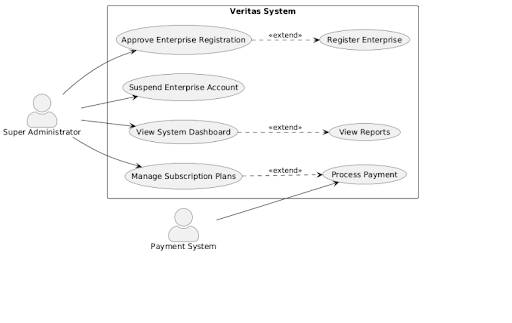
\includegraphics[height=0.75\textheight]{assets/uc_diagrams/uc_super_admin.png}
    \end{center}
\end{frame}

% =============================================================================
% Detailed Use Cases
% =============================================================================
\begin{frame}{UC-01: Approve Enterprise Registration}
    \begin{block}{Use Case Details}
        \begin{description}
            \item[Actor] Super Administrator
            \item[Precondition] Enterprise has submitted registration request
            \item[Postcondition] Enterprise account is approved and activated OR rejected with reason
        \end{description}
    \end{block}
    
    \begin{block}{Main Flow}
        \begin{enumerate}
            \item Super Admin logs into system dashboard
            \item System displays pending enterprise registration requests
            \item Super Admin reviews enterprise details (company info, contact, requested plan)
            \item Super Admin approves or rejects request
            \item If approved: System provisions tenant environment, generates credentials
            \item System sends notification email to enterprise
        \end{enumerate}
    \end{block}
\end{frame}

\begin{frame}{UC-08: Create Exam}
    \begin{center}
        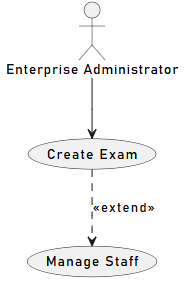
\includegraphics[width=0.7\textwidth]{assets/uc_diagrams/uc_create_exam.png}
    \end{center}
    
    \begin{block}{Key Features}
        \begin{itemize}
            \item Multi-step wizard for comprehensive exam configuration
            \item Question bank selection with targeted randomization
            \item Support for MCQ, True/False, Short Answer, Essay questions
            \item Configurable duration, passing score, negative marking
        \end{itemize}
    \end{block}
\end{frame}

\begin{frame}{UC-18: Start Exam (Candidate Flow)}
    \begin{center}
        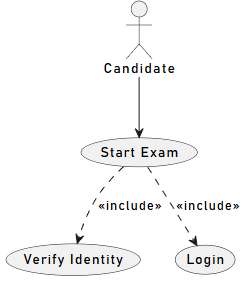
\includegraphics[width=0.65\textwidth]{assets/uc_diagrams/uc_start_exam.png}
    \end{center}
    
    \begin{block}{Critical Steps}
        \begin{enumerate}
            \item Candidate authenticates with enterprise token/ID
            \item System verifies exam schedule and candidate eligibility
            \item Candidate completes identity verification (facial capture)
            \item System performs system check (camera, browser compatibility)
            \item Exam interface loads in fullscreen mode with proctoring active
        \end{enumerate}
    \end{block}
\end{frame}

% =============================================================================
% Sequence Diagrams
% =============================================================================
\begin{frame}{Sequence Diagrams: Overview}
    \textbf{Sequence diagrams illustrate interactions between actors and system for key use cases}
    
    \begin{block}{Categories Covered}
        \begin{enumerate}
            \item \textbf{Enterprise Onboarding \& Lifecycle}
            \begin{itemize}
                \item Enterprise Registration \& Approval Workflow
                \item Subscription Payment \& Dunning Process
            \end{itemize}
            
            \item \textbf{Authentication \& Security}
            \begin{itemize}
                \item Candidate Login with Face Verification
                \item Session Timeout \& Re-authentication
            \end{itemize}
            
            \item \textbf{Examination Management}
            \begin{itemize}
                \item Bulk Enrollment \& Token Generation
                \item Exam Configuration (Targeted Randomization)
            \end{itemize}
        \end{enumerate}
    \end{block}
\end{frame}

\begin{frame}{Sequence Diagrams: Overview (continued)}
    \begin{block}{Categories Covered (continued)}
        \begin{enumerate}
            \setcounter{enumi}{3}
            \item \textbf{Candidate Exam Experience}
            \begin{itemize}
                \item Answer Auto-Save \& Sync
            \end{itemize}
            
            \item \textbf{AI Proctoring \& Monitoring}
            \begin{itemize}
                \item Proctoring Event Loop
            \end{itemize}
            
            \item \textbf{Grading \& Reporting}
            \begin{itemize}
                \item Hybrid Grading Workflow
                \item Async Report Generation
            \end{itemize}
        \end{enumerate}
    \end{block}
    
    \vspace{0.3cm}
    \textit{Each diagram maps to specific functional requirements}
\end{frame}

\begin{frame}{SD: Enterprise Registration \& Approval}
    \begin{center}
        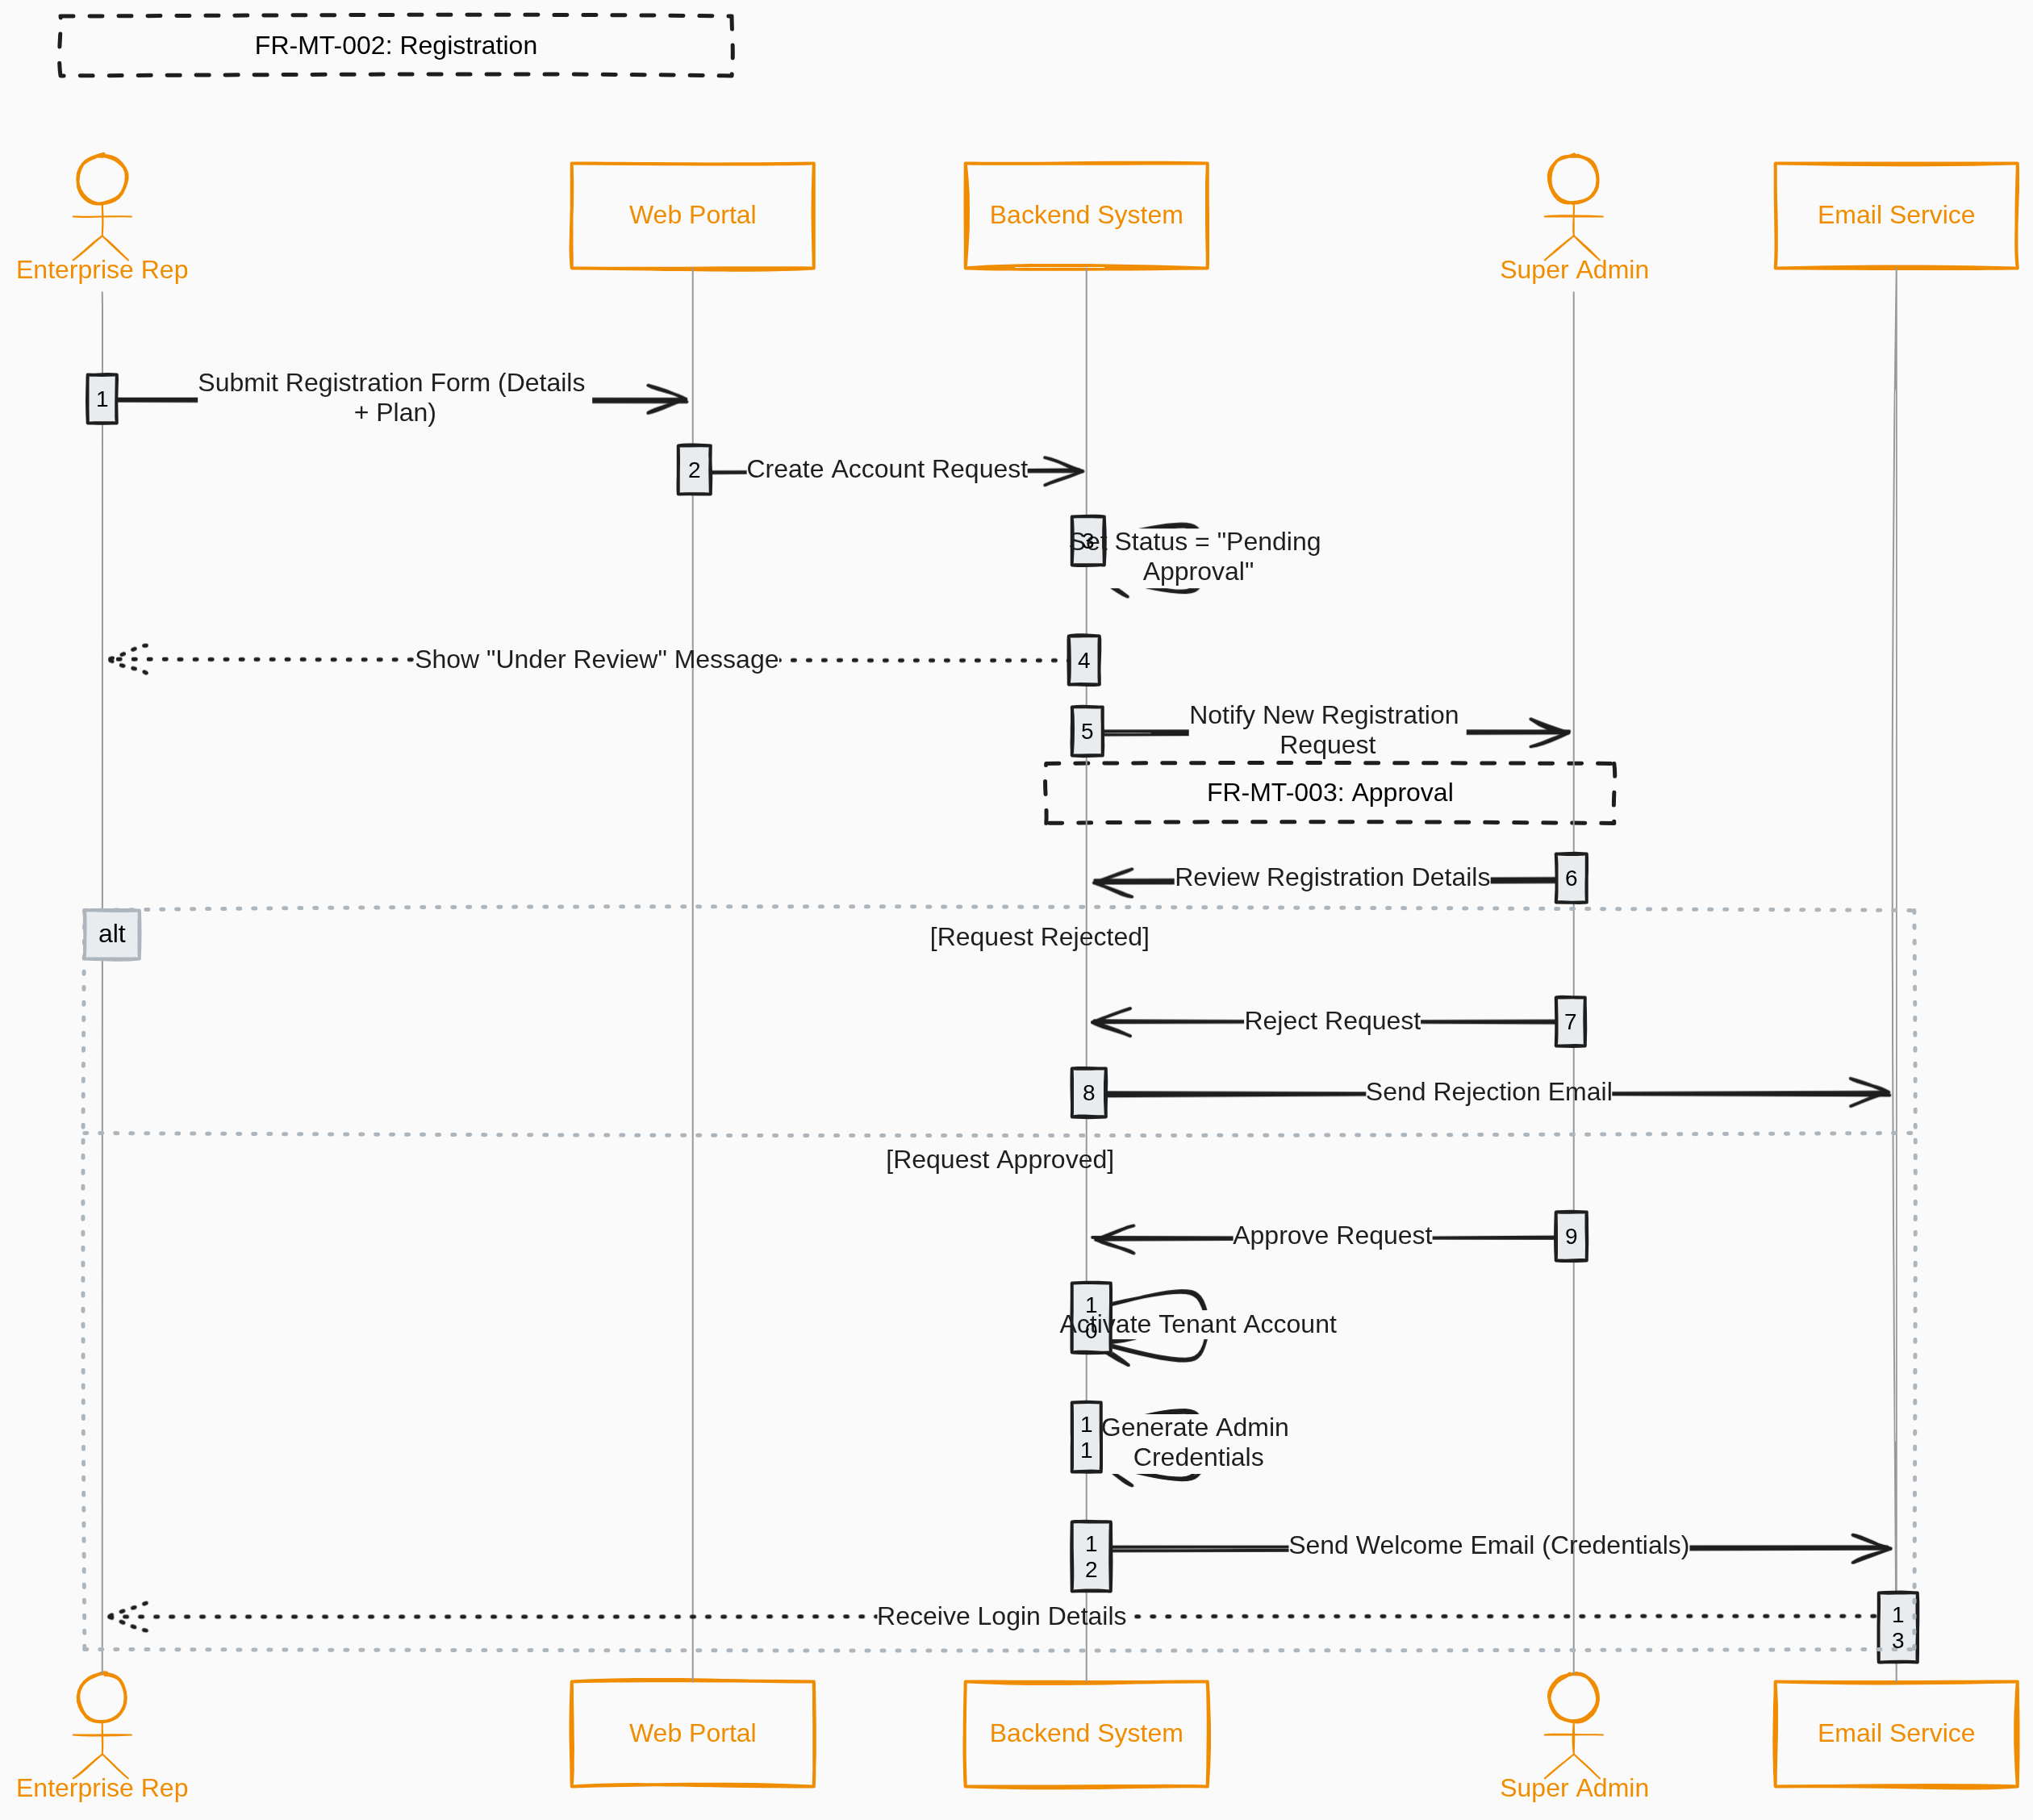
\includegraphics[width=0.9\textwidth]{assets/seq_diagrams/Enterprise Registration.png}
    \end{center}
    
    \textbf{Implements:} FR-MT-002, FR-MT-003
\end{frame}

\begin{frame}{SD: Subscription Payment \& Dunning}
    \begin{center}
        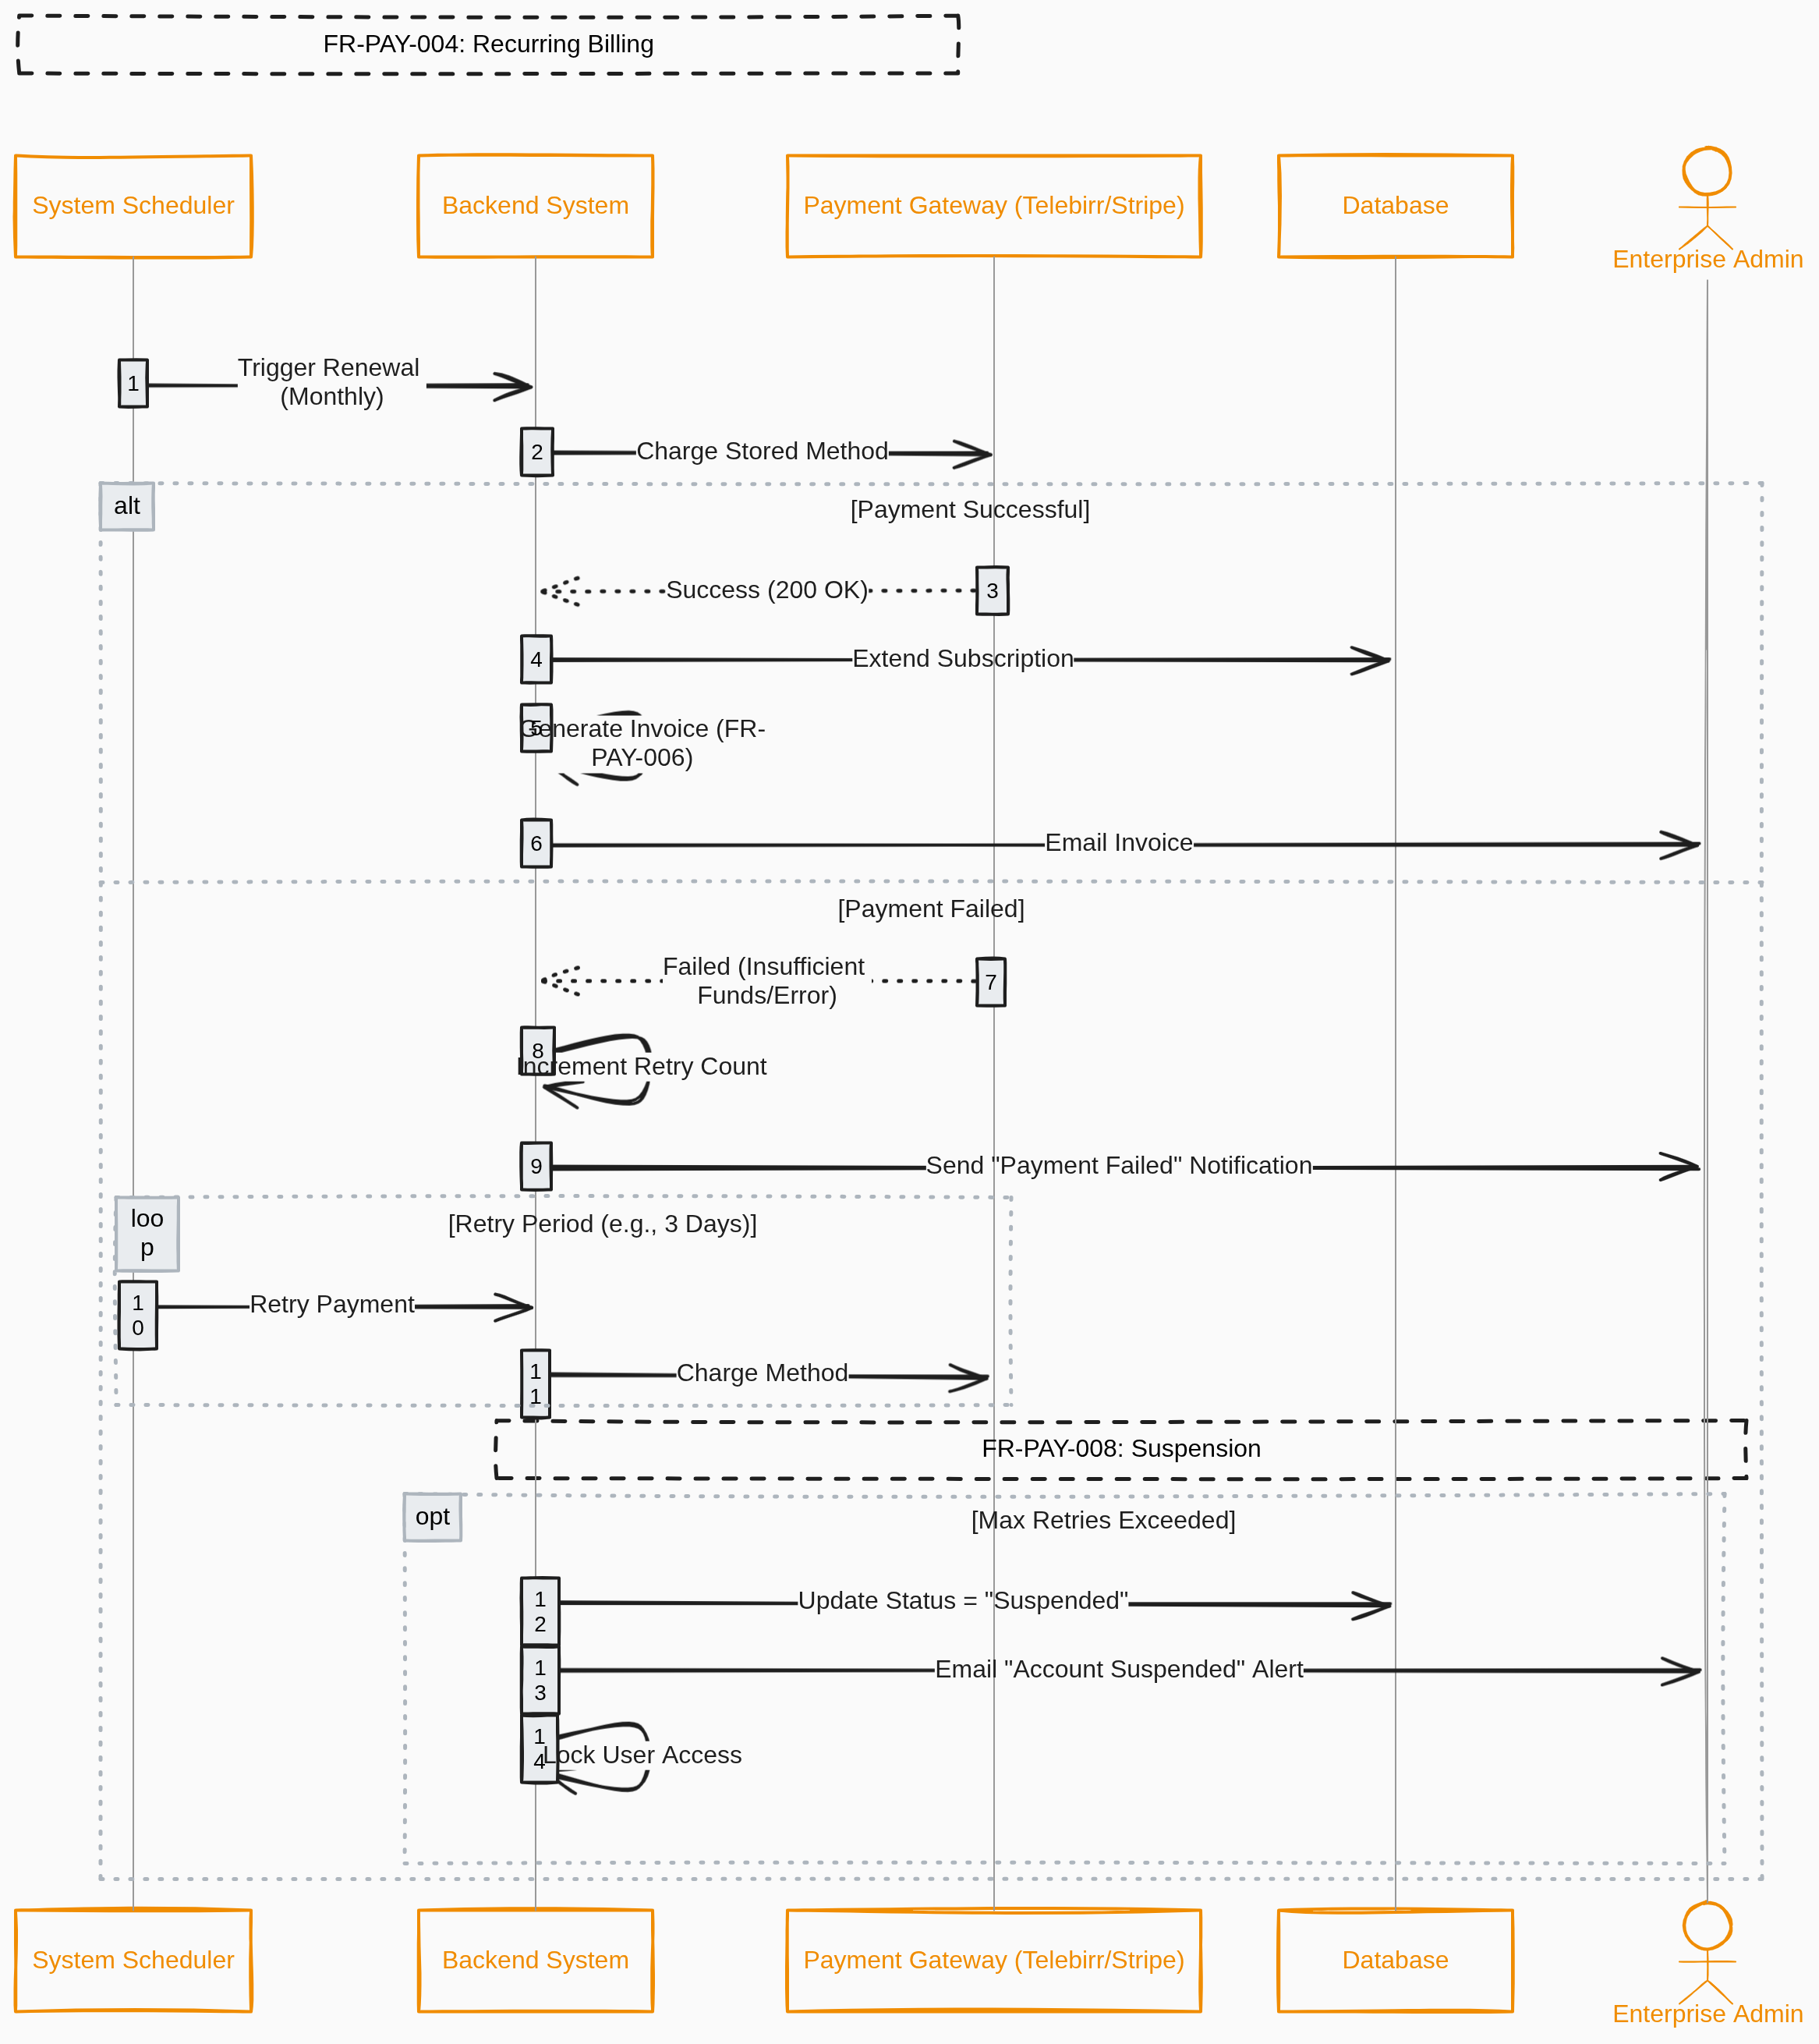
\includegraphics[width=0.9\textwidth]{assets/seq_diagrams/Subscription Payment & Dunning (Suspension).png}
    \end{center}
    
    \textbf{Implements:} FR-PAY-004, FR-PAY-008 \\
    \textit{Financial lifecycle: billing, retry loop, account suspension}
\end{frame}

\begin{frame}{SD: Candidate Login with Face Verification}
    \begin{center}
        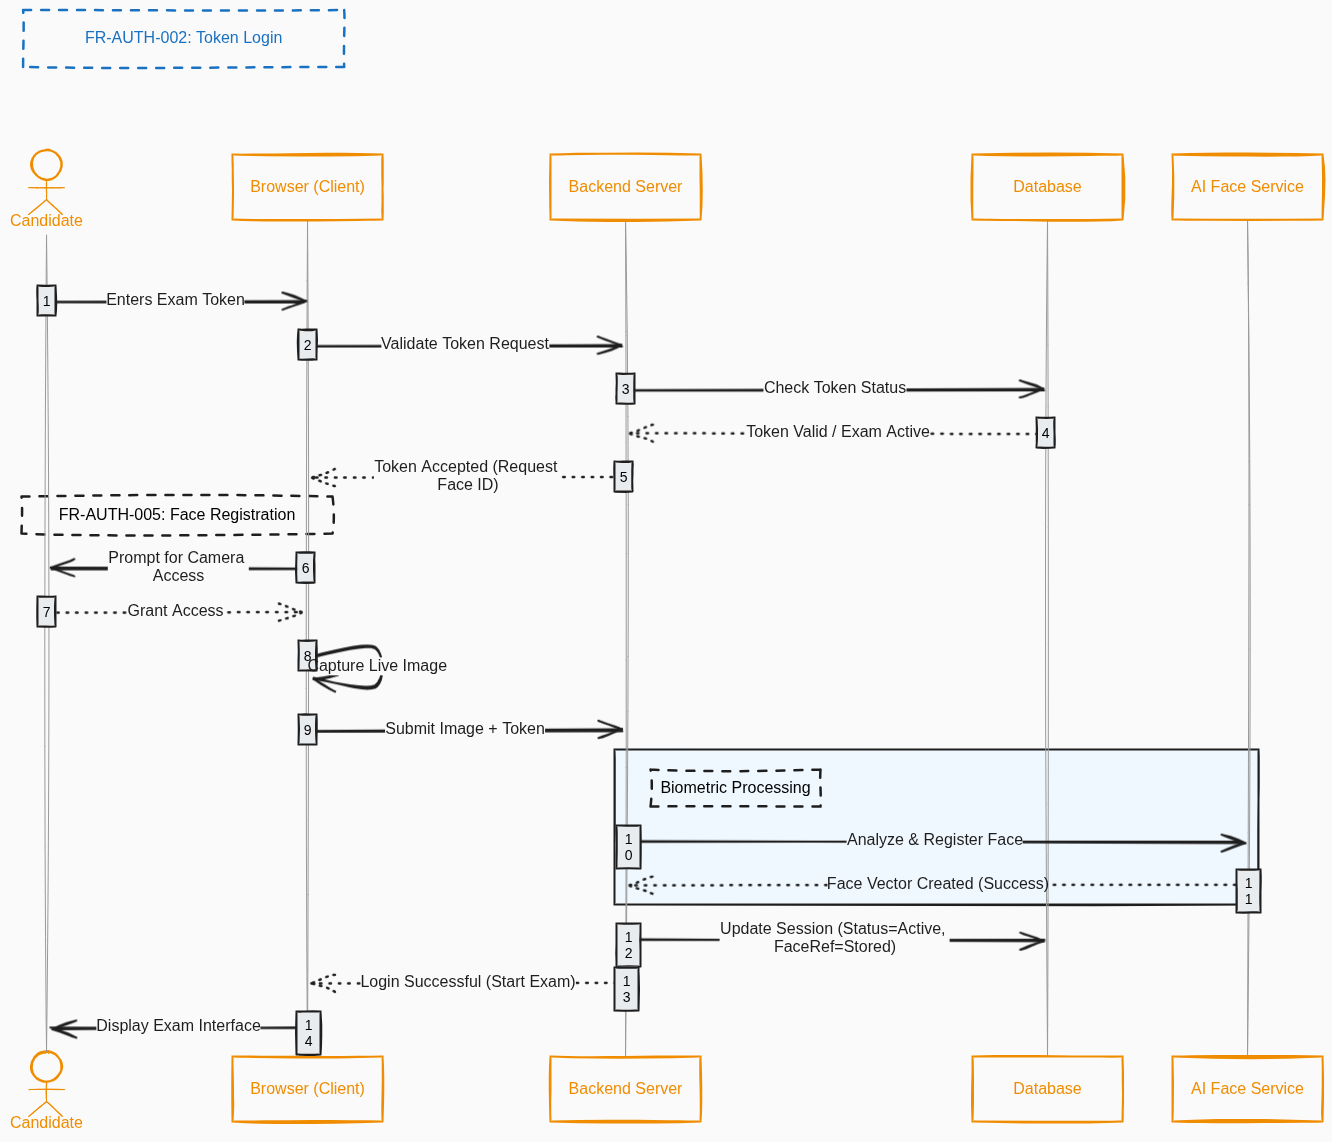
\includegraphics[width=0.9\textwidth]{assets/seq_diagrams/FR-2.png}
    \end{center}
    
    \textbf{Implements:} FR-AUTH-002, FR-AUTH-005 \\
    \textit{Multi-factor authentication to eliminate impersonation}
\end{frame}

\begin{frame}{SD: Session Timeout \& Re-authentication}
    \begin{center}
        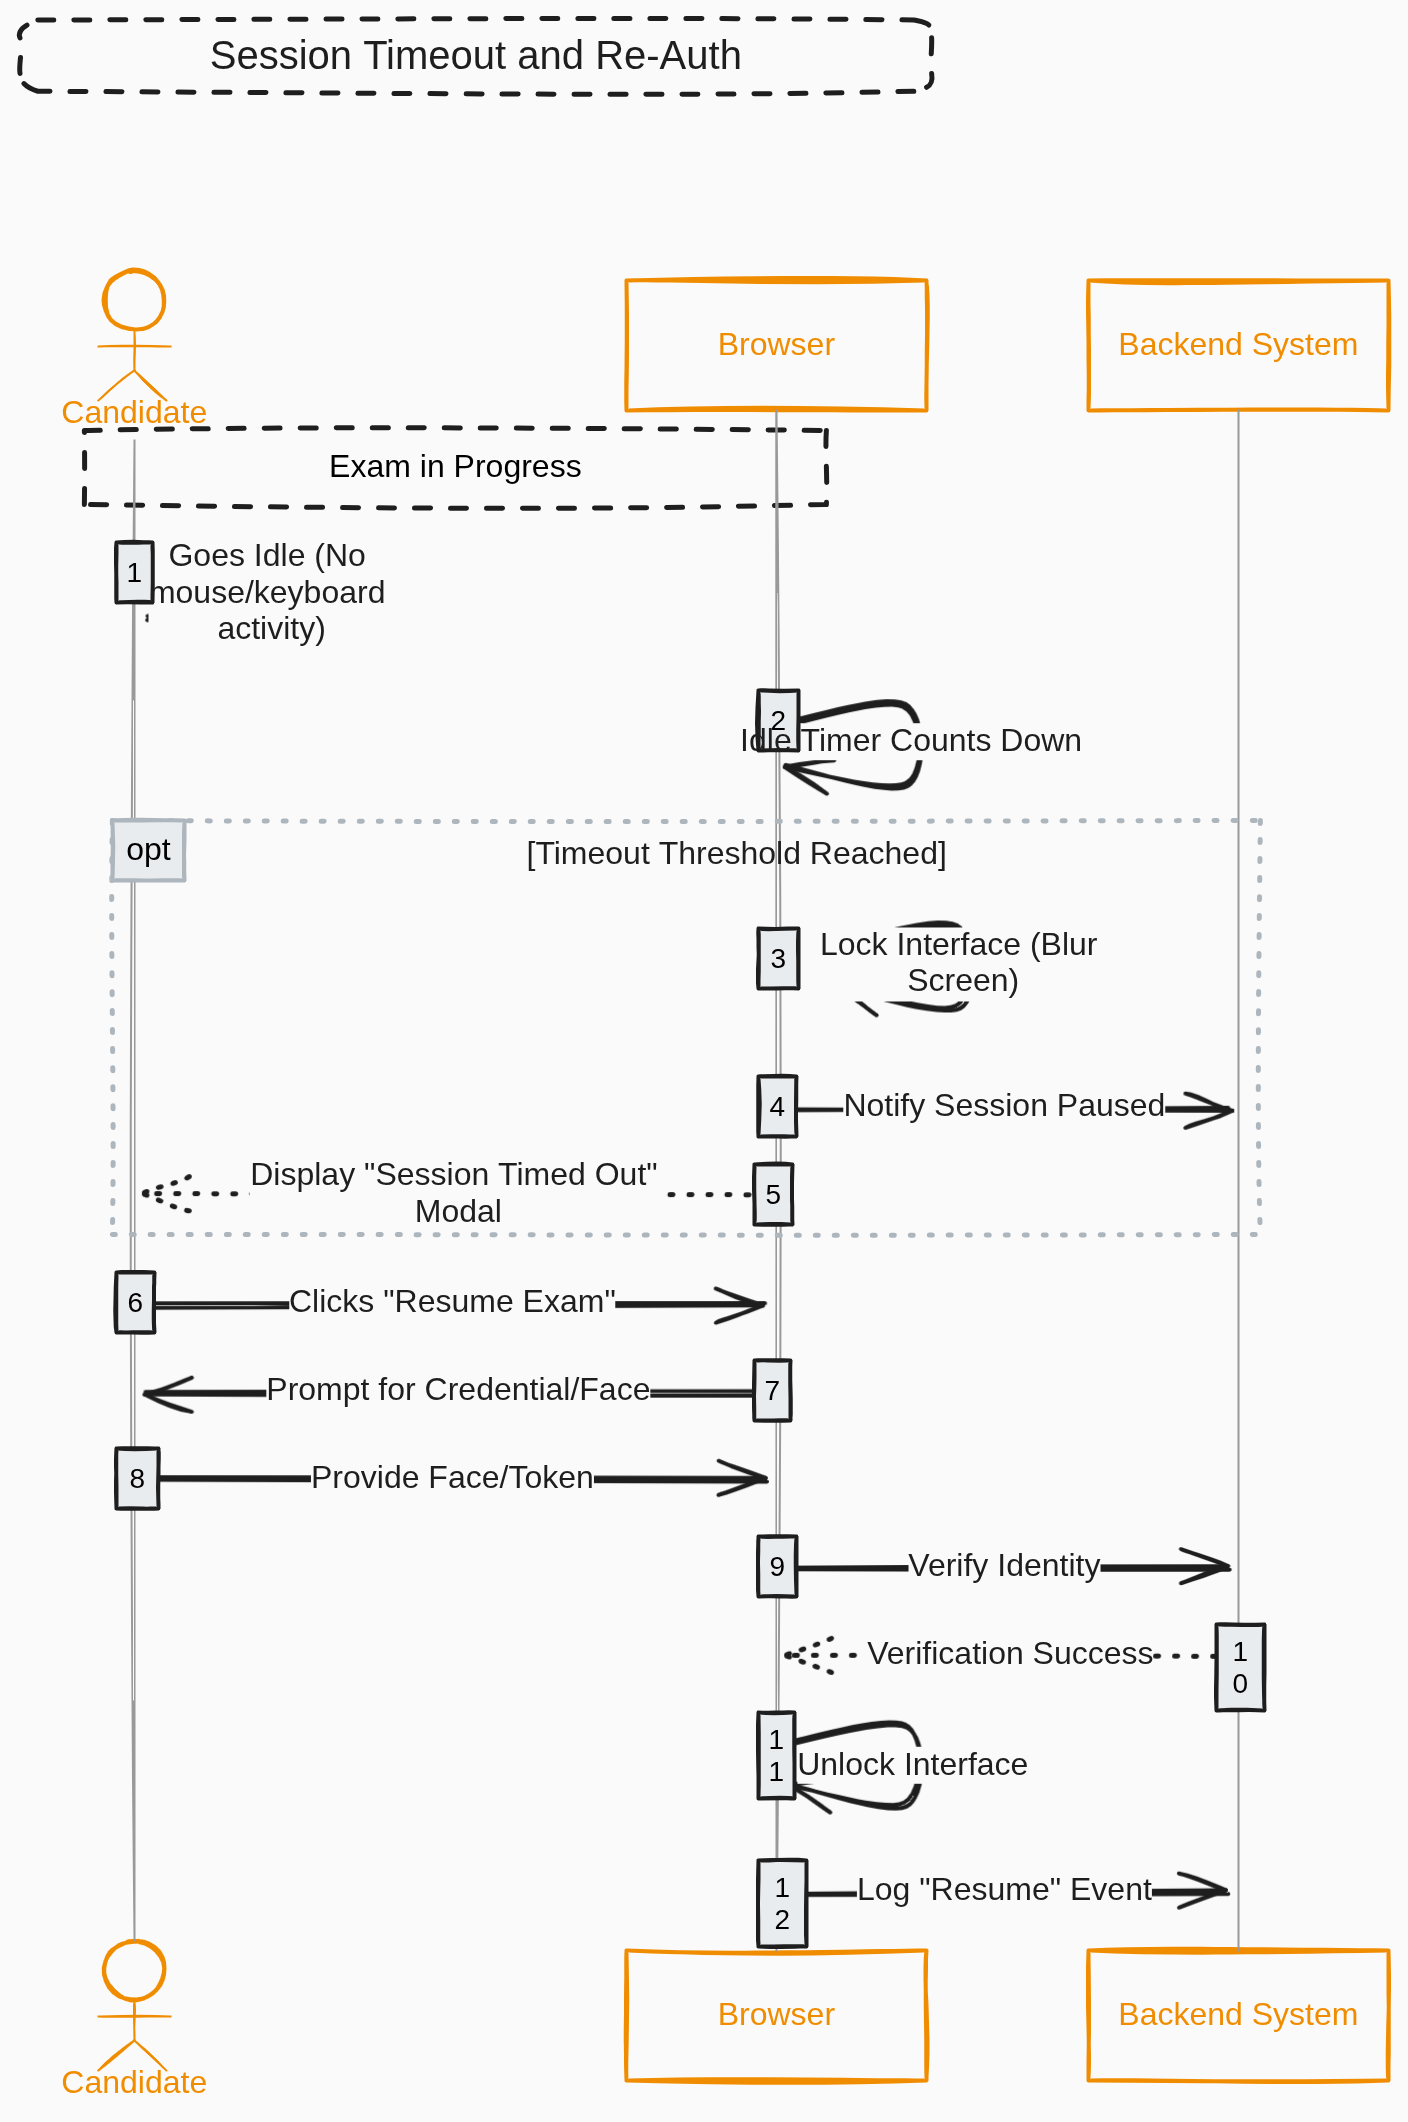
\includegraphics[width=0.75\textwidth]{assets/seq_diagrams/Session Timeout and Re-Auth.png}
    \end{center}
    
    \textbf{Implements:} FR-AUTH-007 \\
    \textit{Security response to user inactivity - prevents exploitation of unattended workstation}
\end{frame}

\begin{frame}{SD: Bulk Enrollment \& Token Generation}
    \begin{center}
        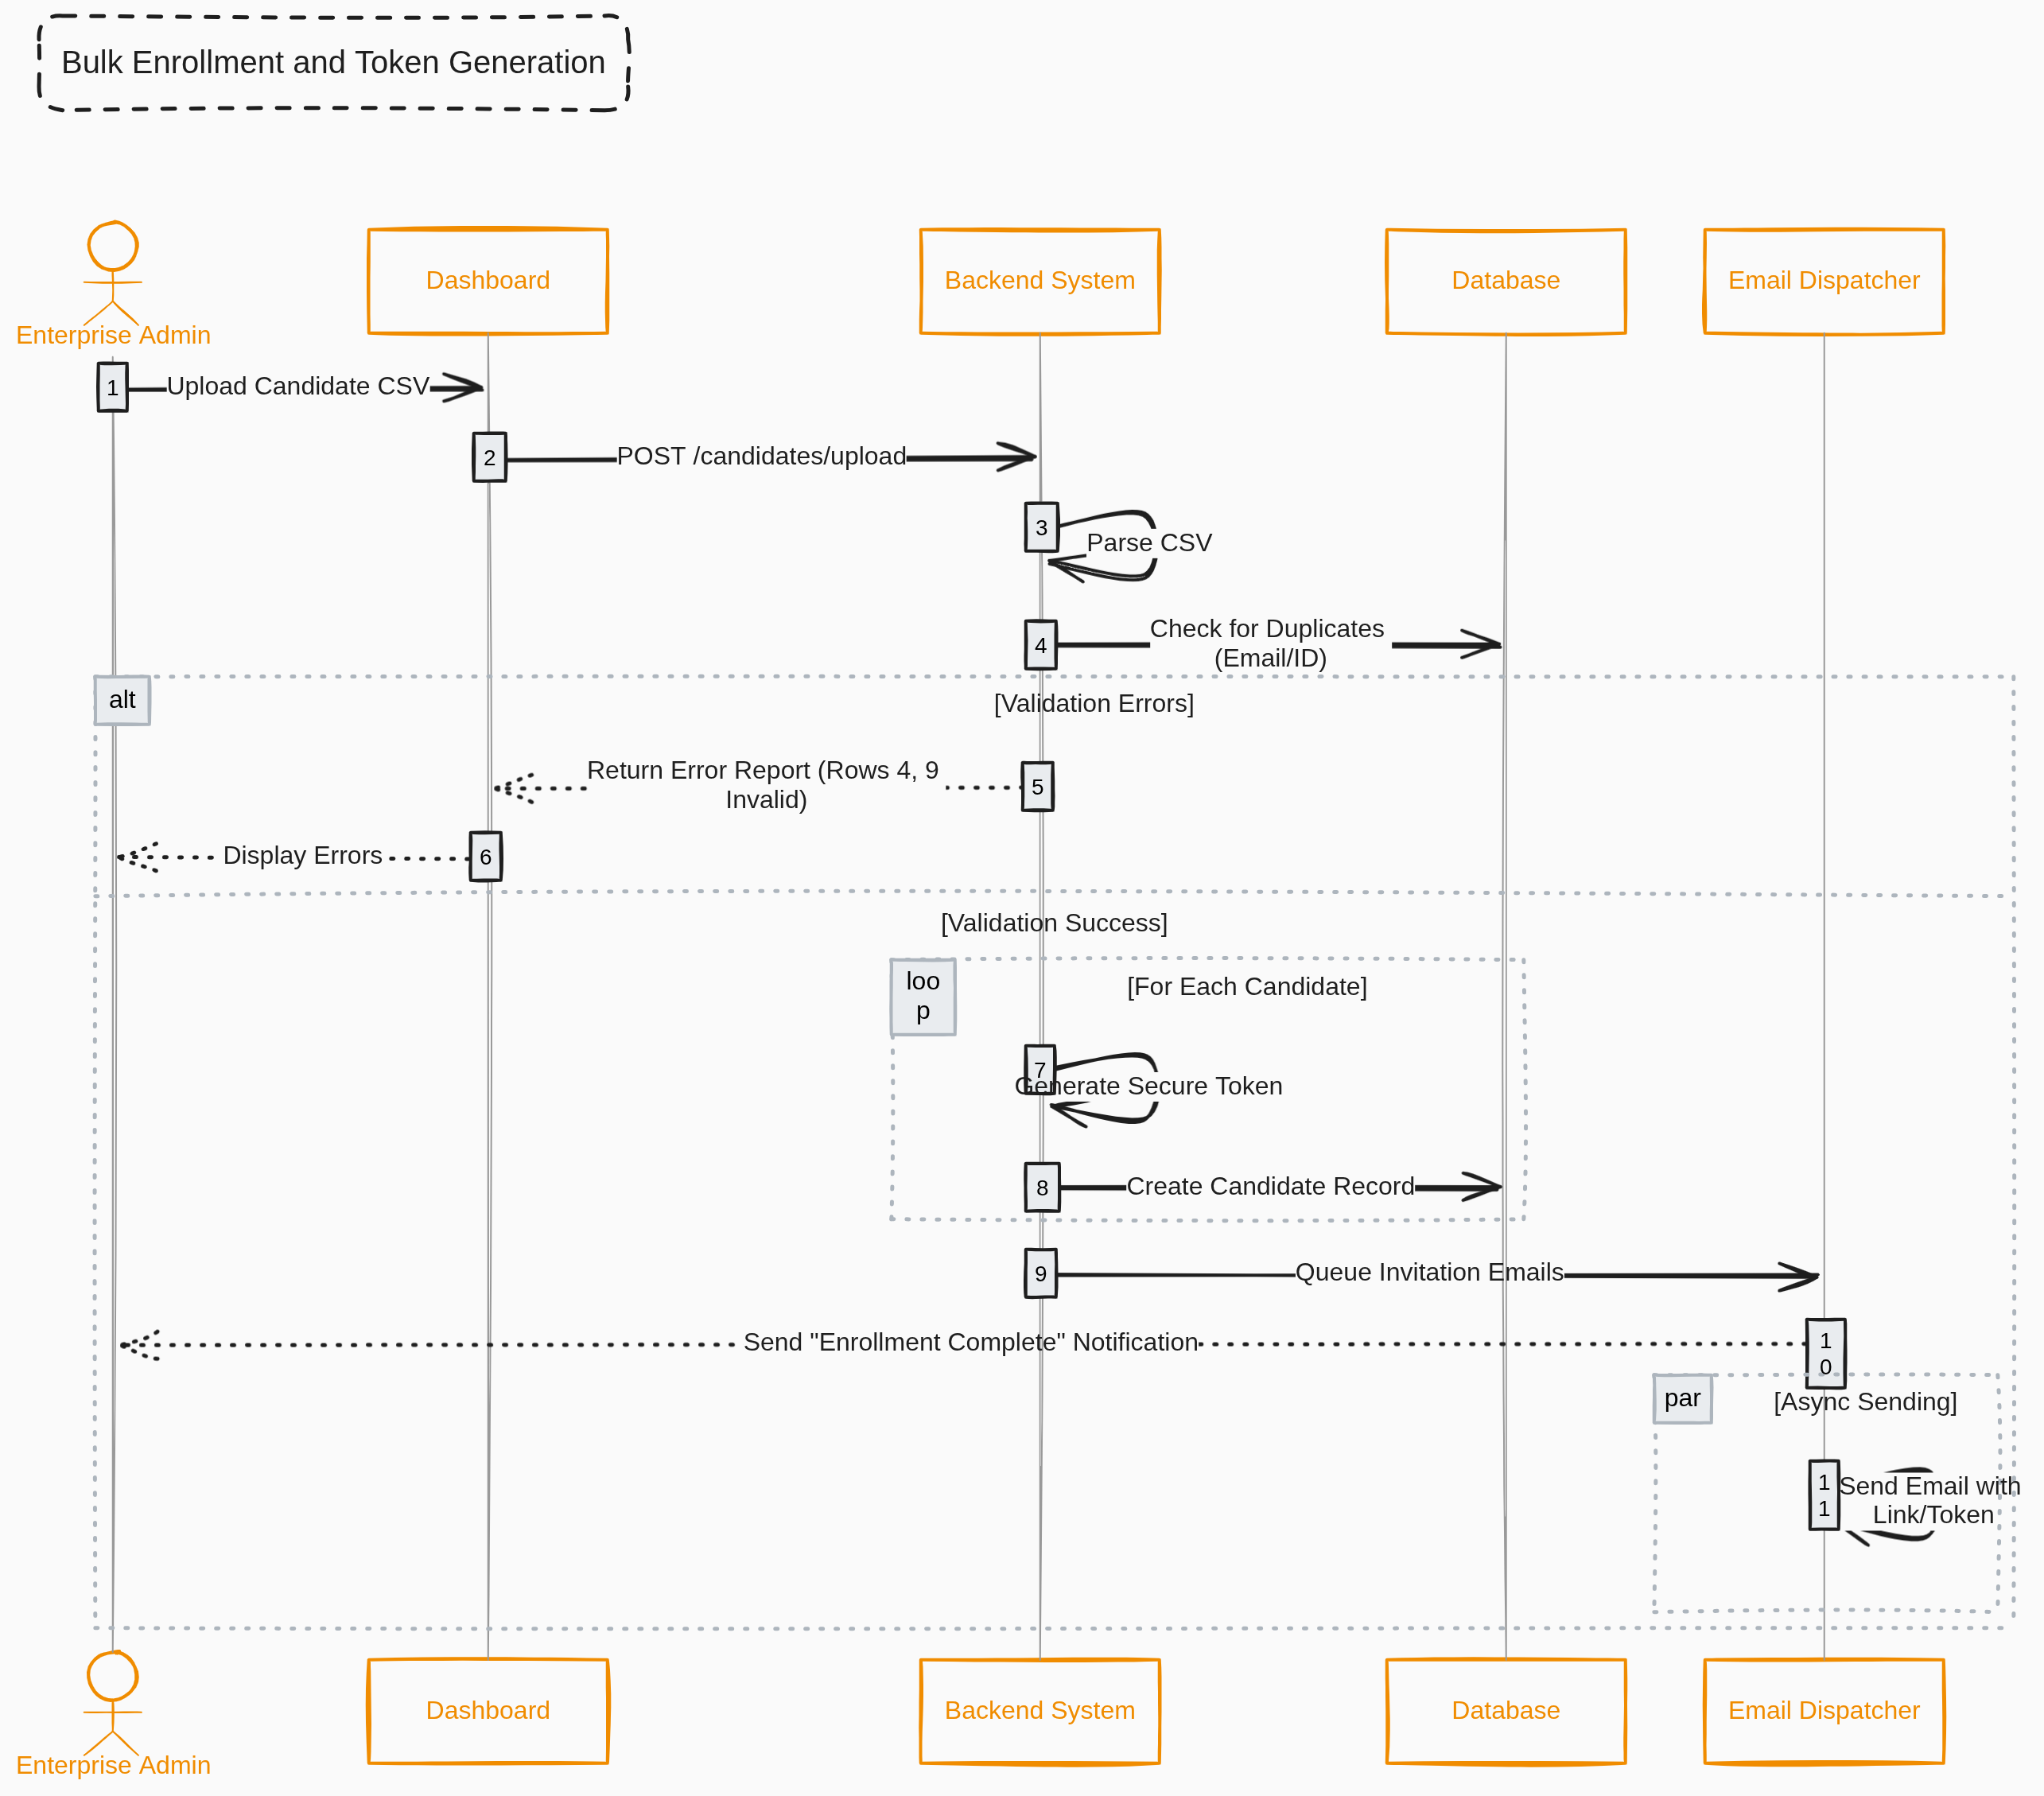
\includegraphics[width=0.9\textwidth]{assets/seq_diagrams/Bulk Enrollment and Token Gen.png}
    \end{center}
    
    \textbf{Implements:} FR-EXM-004 \\
    \textit{High-volume data processing for large exams: CSV upload, validation, token generation, email dispatch}
\end{frame}

\begin{frame}{SD: Exam Configuration (Targeted Randomization)}
    \begin{center}
        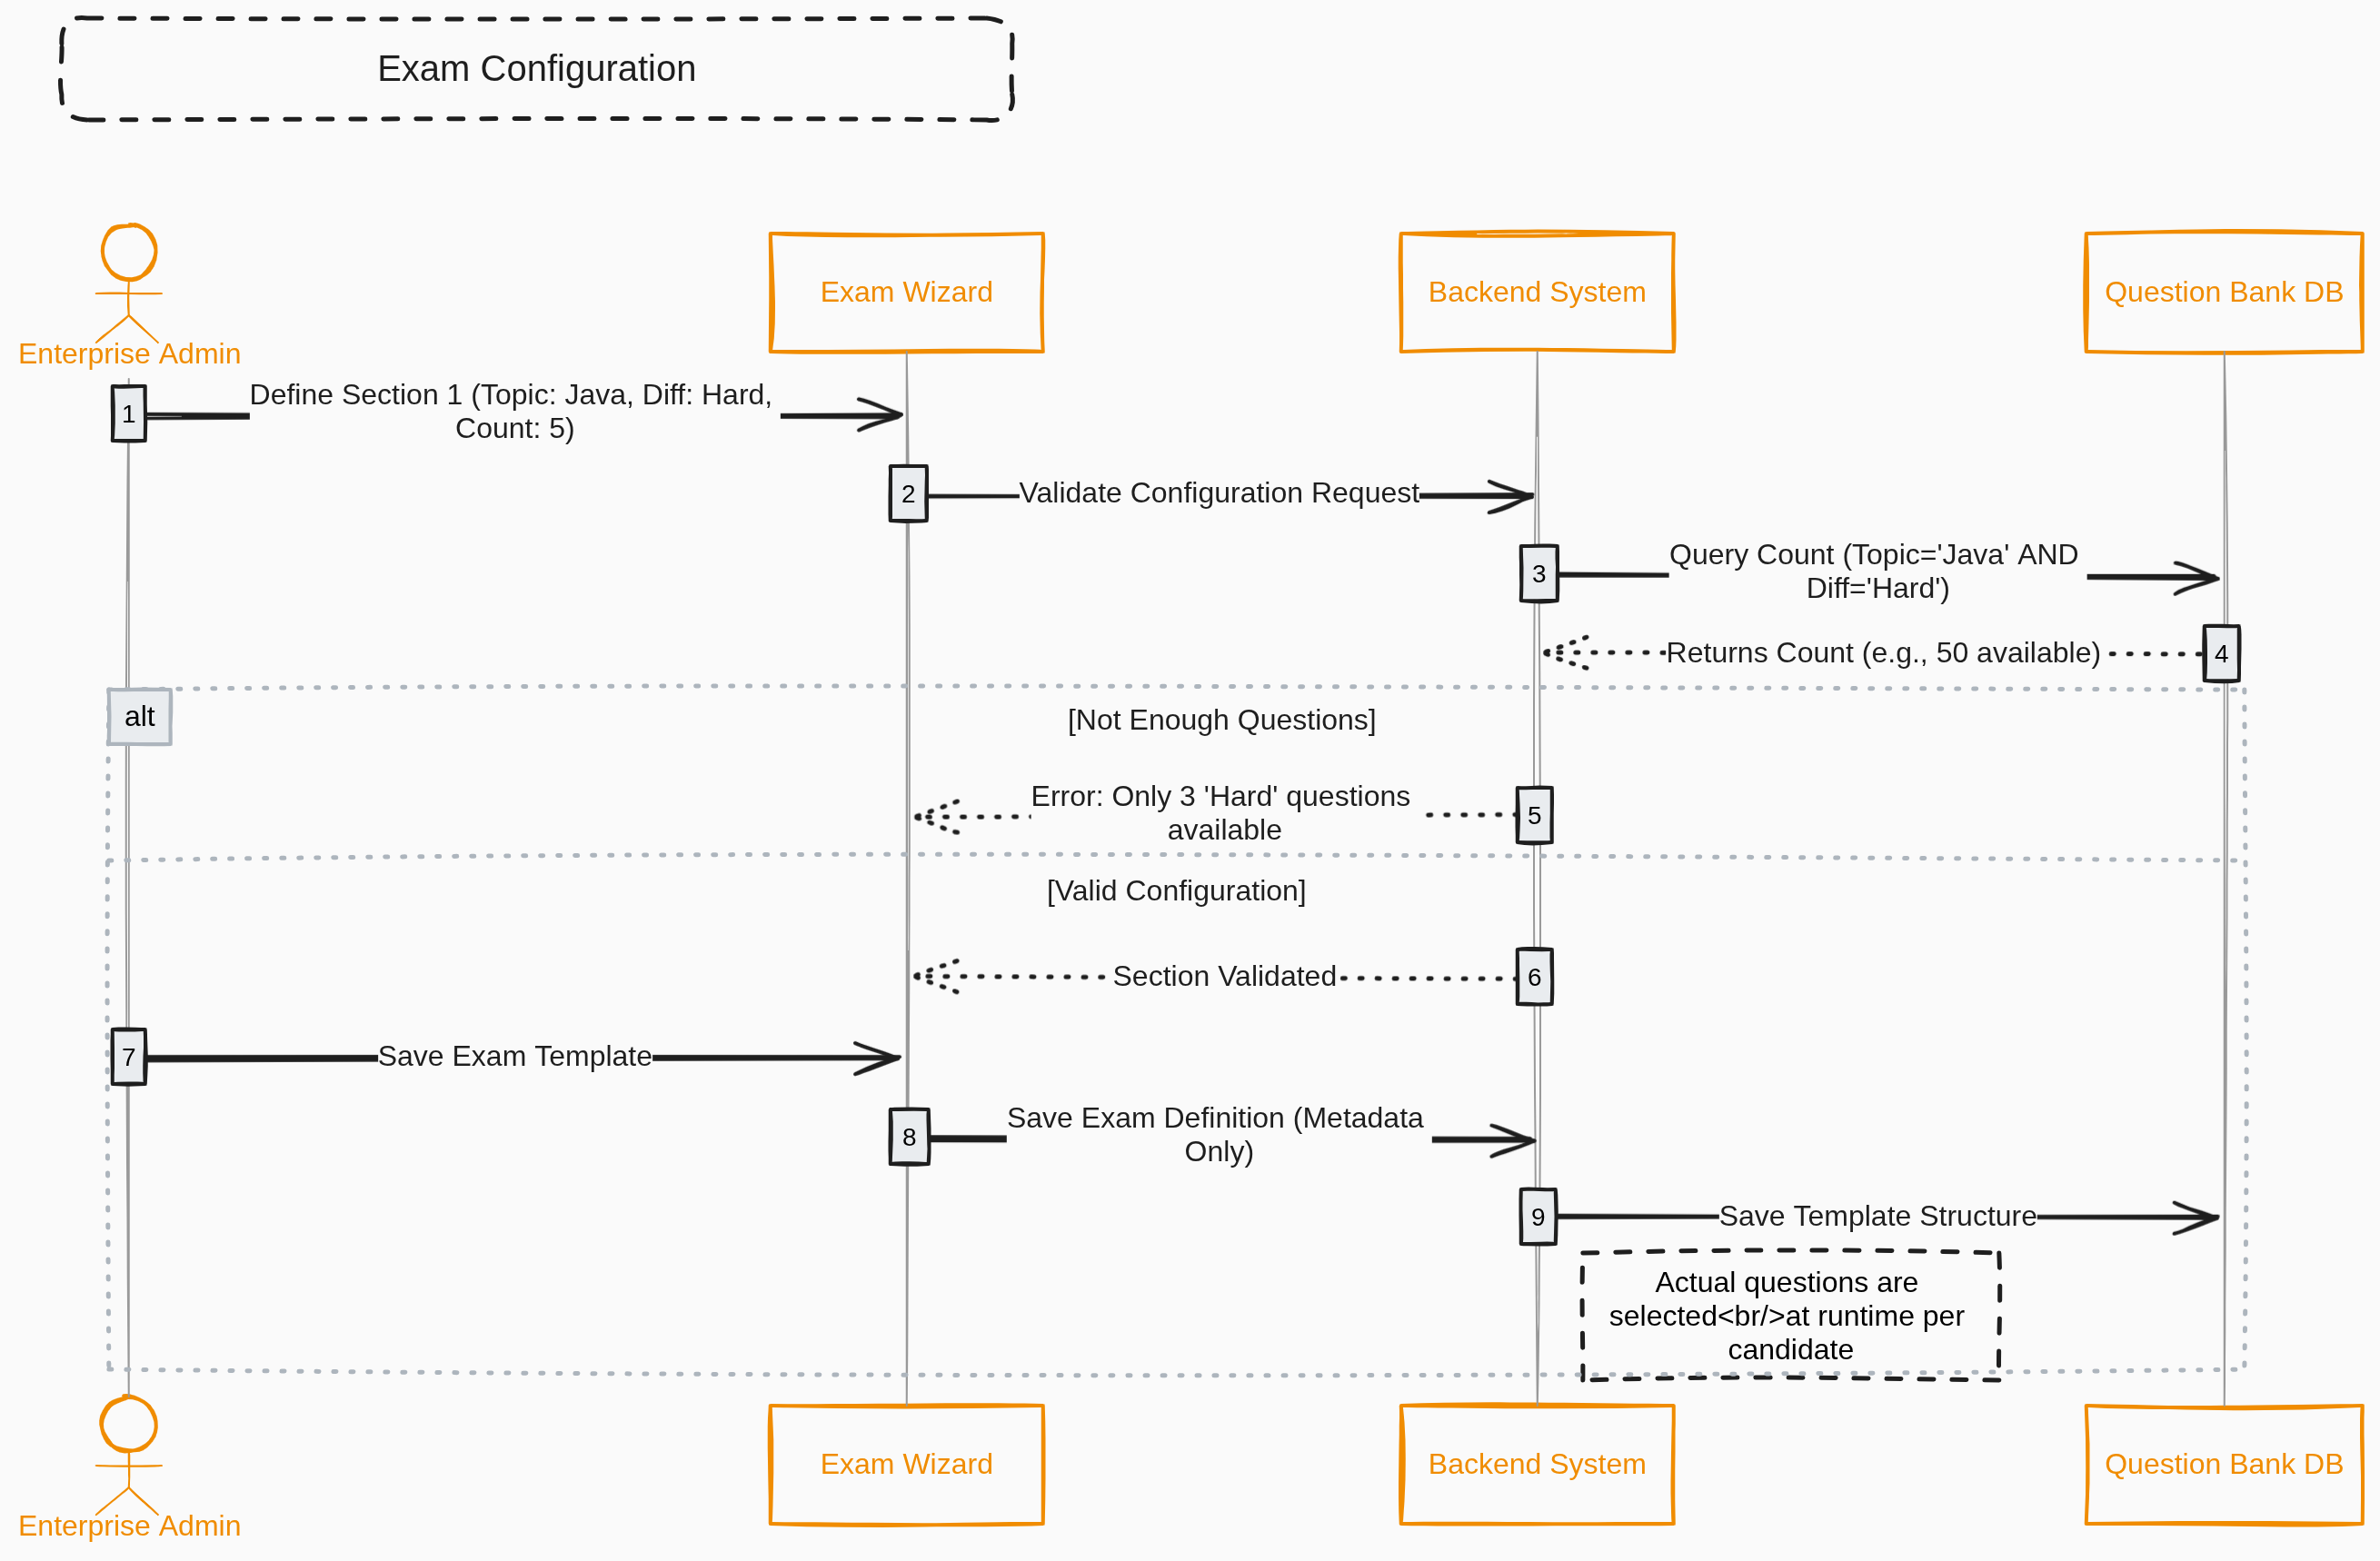
\includegraphics[width=0.9\textwidth]{assets/seq_diagrams/Exam Configuration.png}
    \end{center}
    
    \textbf{Implements:} FR-EXM-002 \\
    \textit{Dynamic, randomized exams: Admin defines criteria, system validates question bank, saves template}
\end{frame}

\begin{frame}{SD: Answer Auto-Save \& Sync}
    \begin{center}
        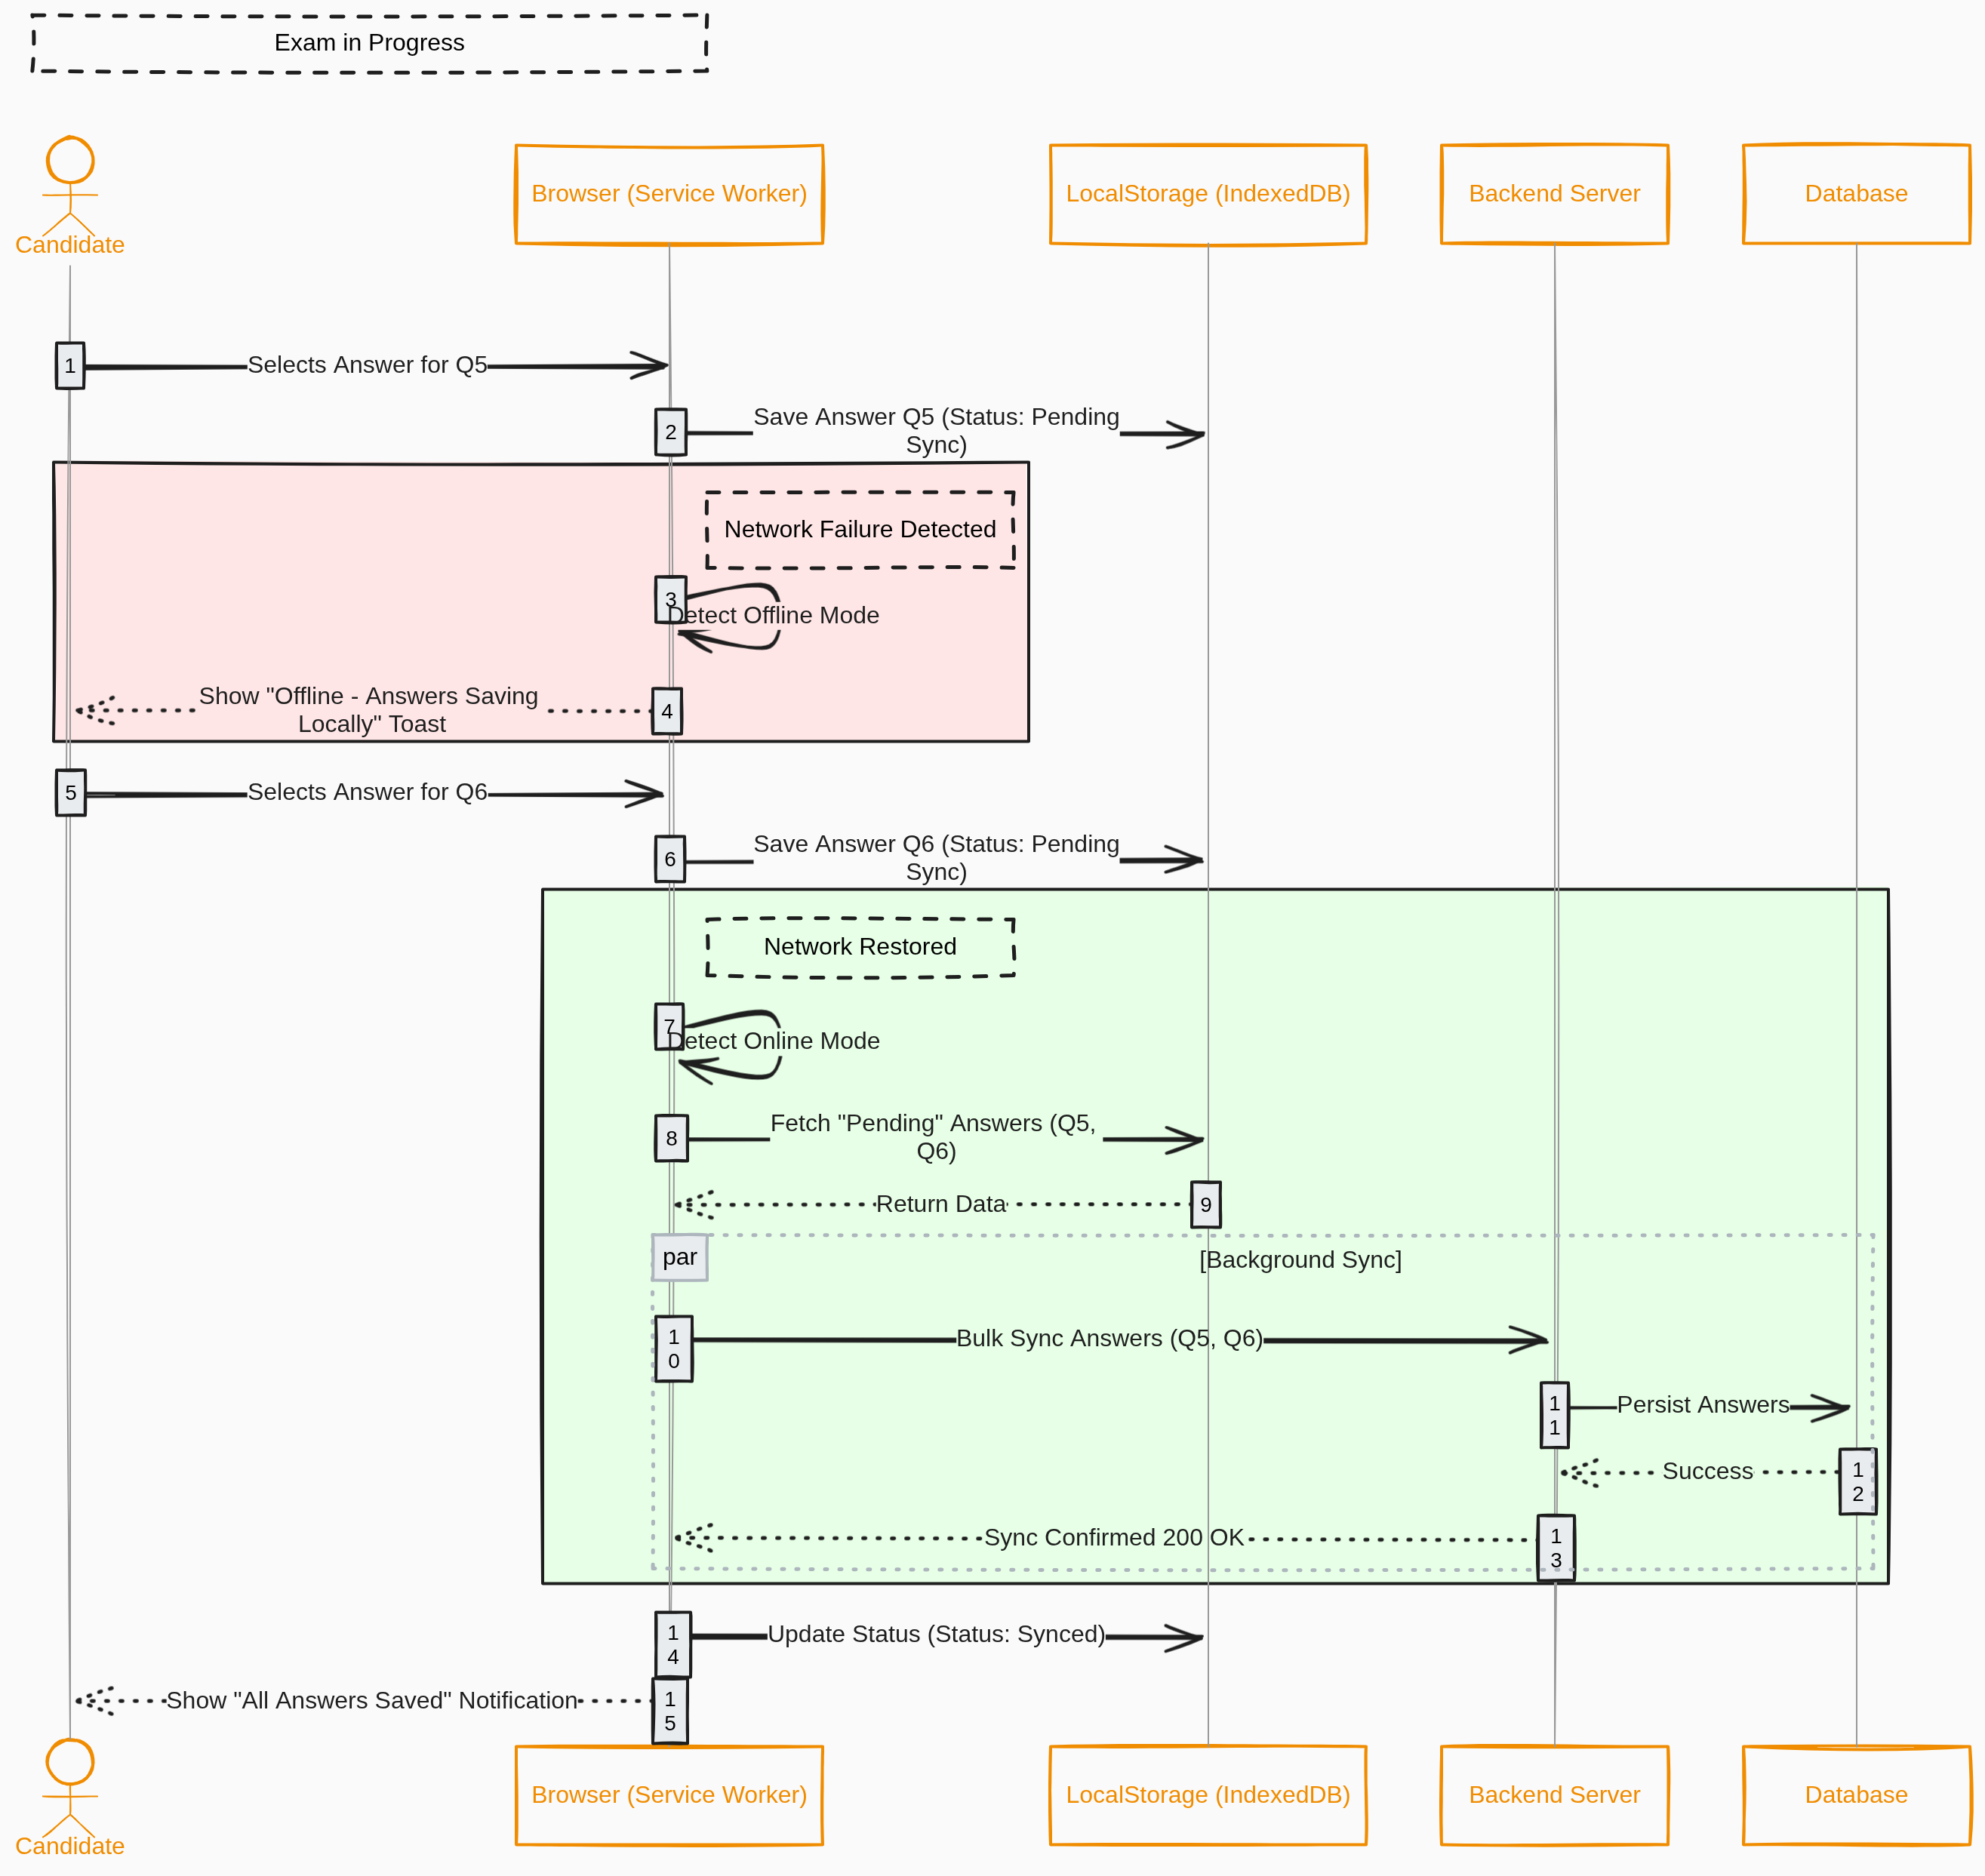
\includegraphics[width=0.9\textwidth]{assets/seq_diagrams/Exam in Progress.png}
    \end{center}
    
    \textbf{Implements:} FR-CAND-004 \\
    \textit{Data synchronization protecting candidate progress: local storage + periodic server sync}
\end{frame}

\begin{frame}{SD: Proctoring Event Loop}
    \begin{center}
        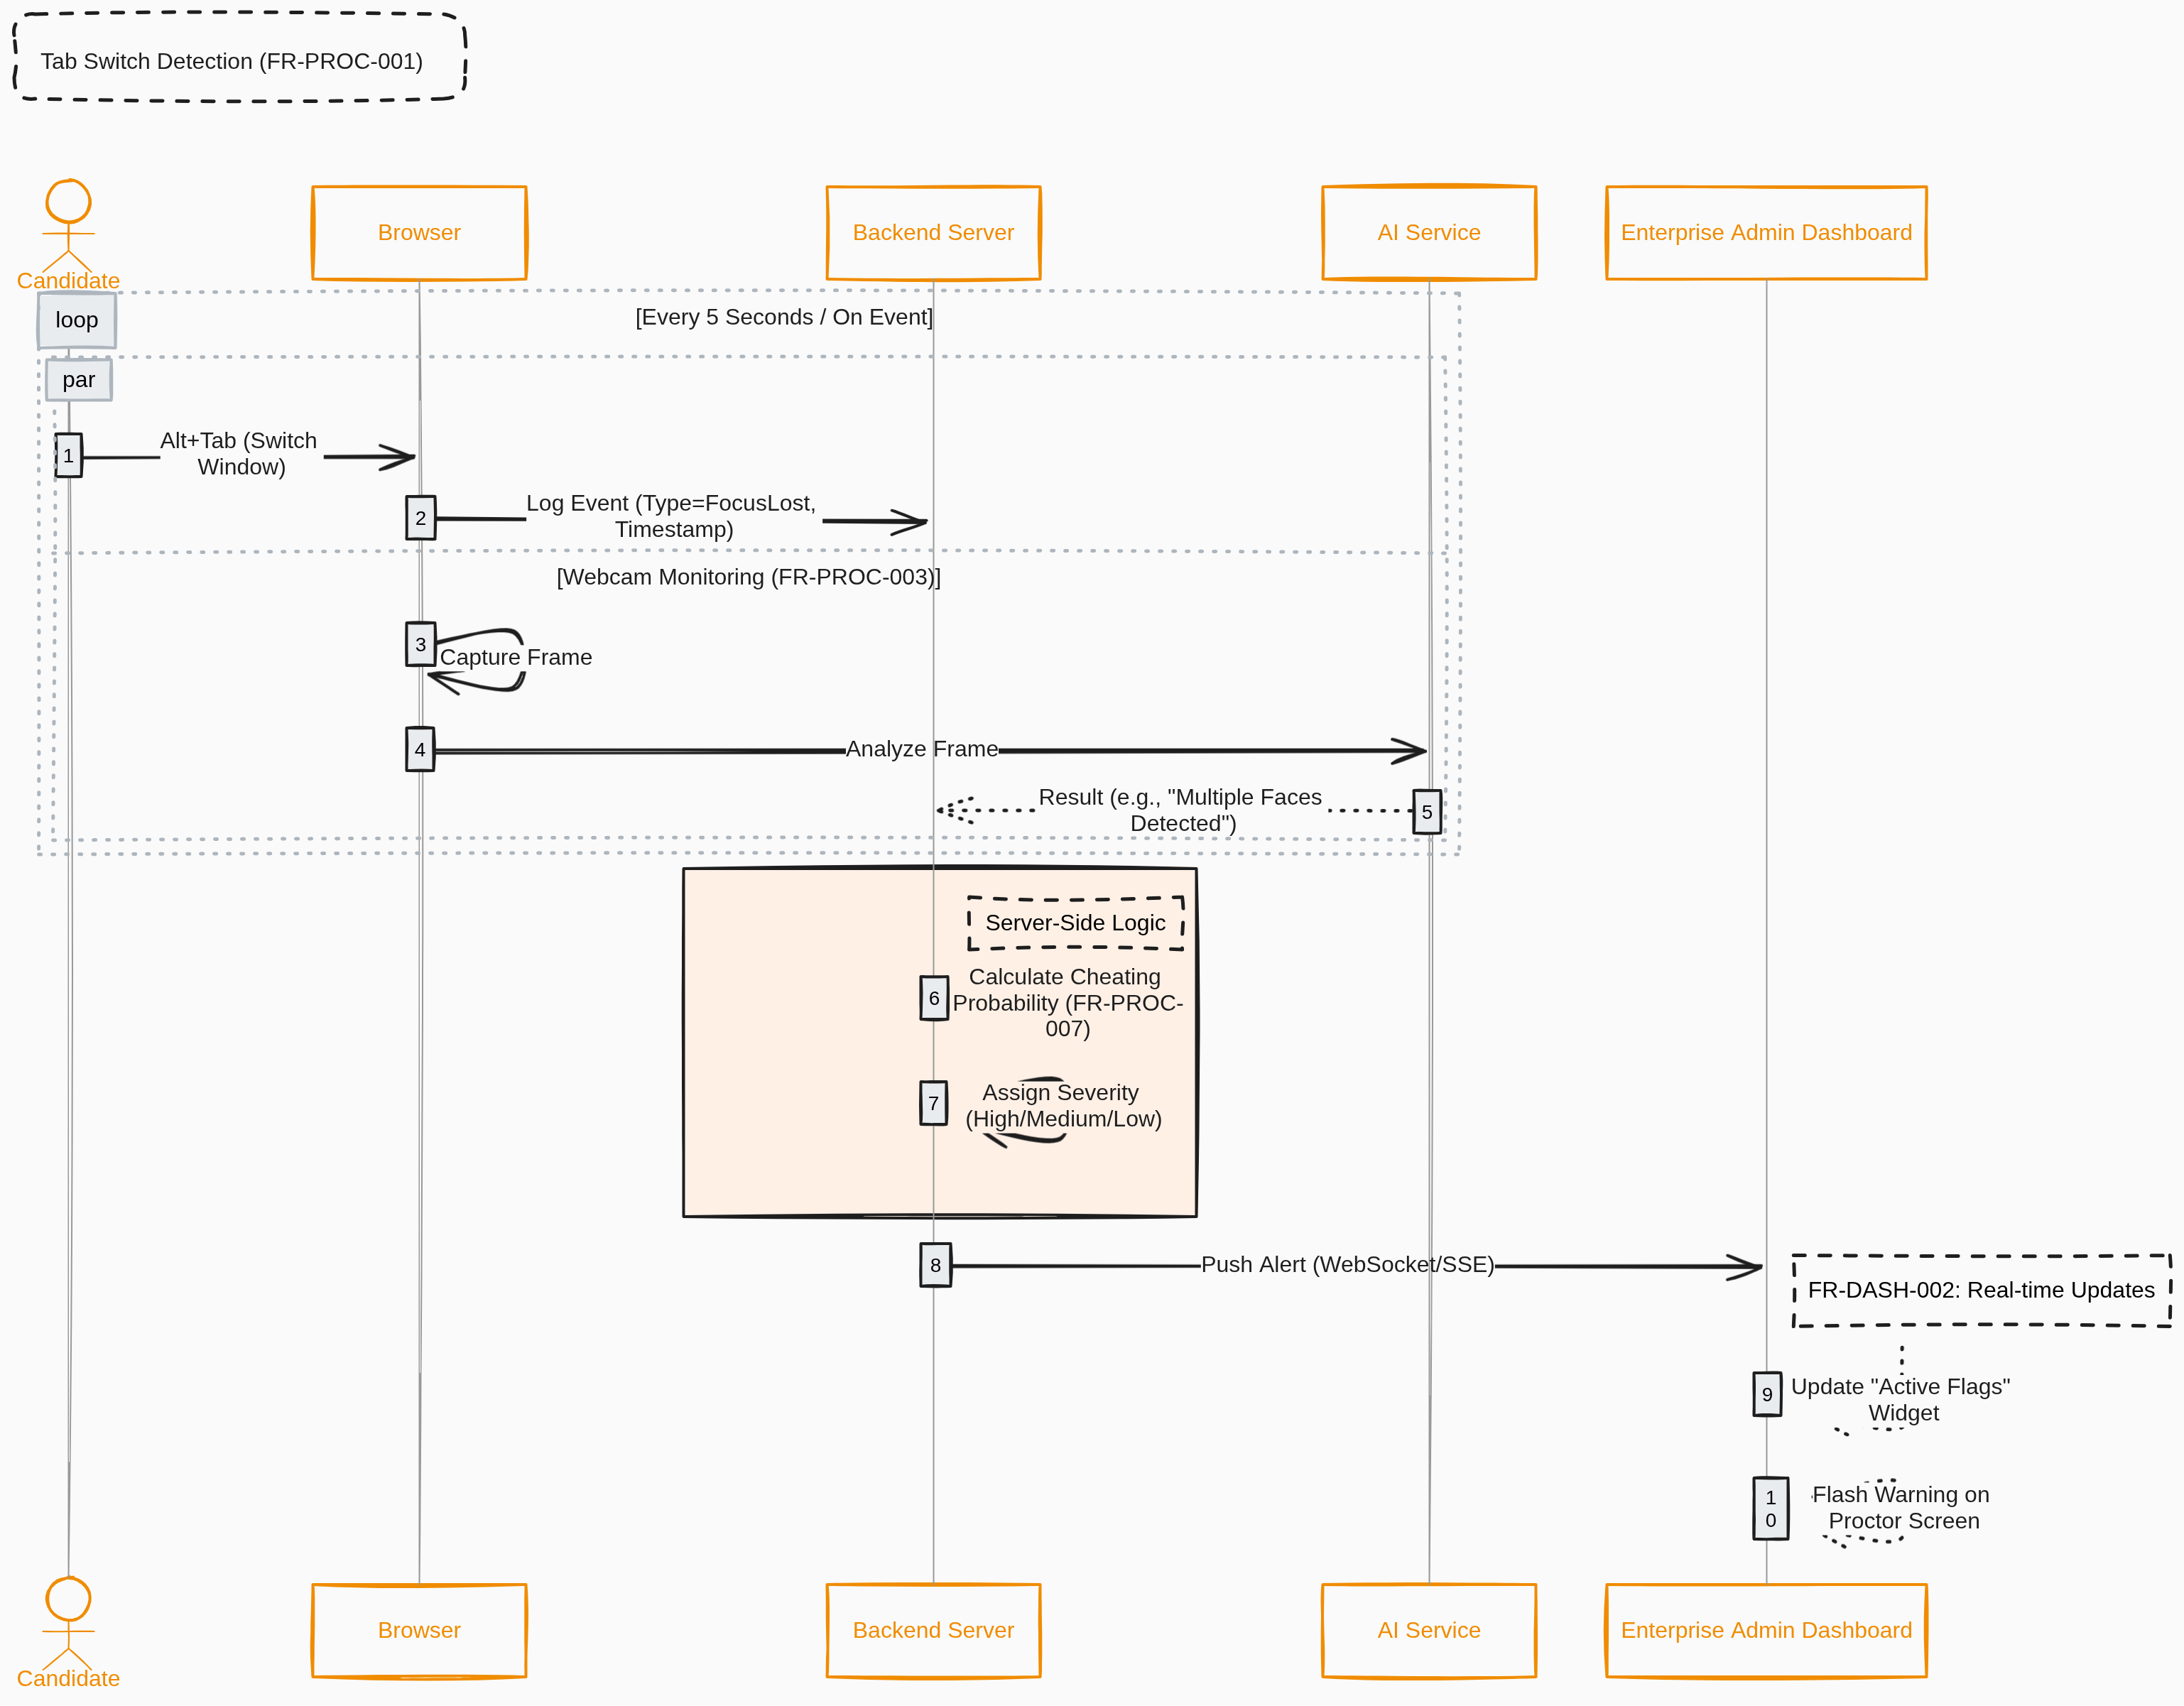
\includegraphics[width=0.9\textwidth]{assets/seq_diagrams/Tab Switch Detection.png}
    \end{center}
    
    \textbf{Implements:} FR-PROC-001, FR-DASH-002 \\
    \textit{Real-time monitoring: browser events + webcam AI analysis → cheating probability score → Admin dashboard}
\end{frame}

\begin{frame}{SD: Hybrid Grading Workflow}
    \begin{center}
        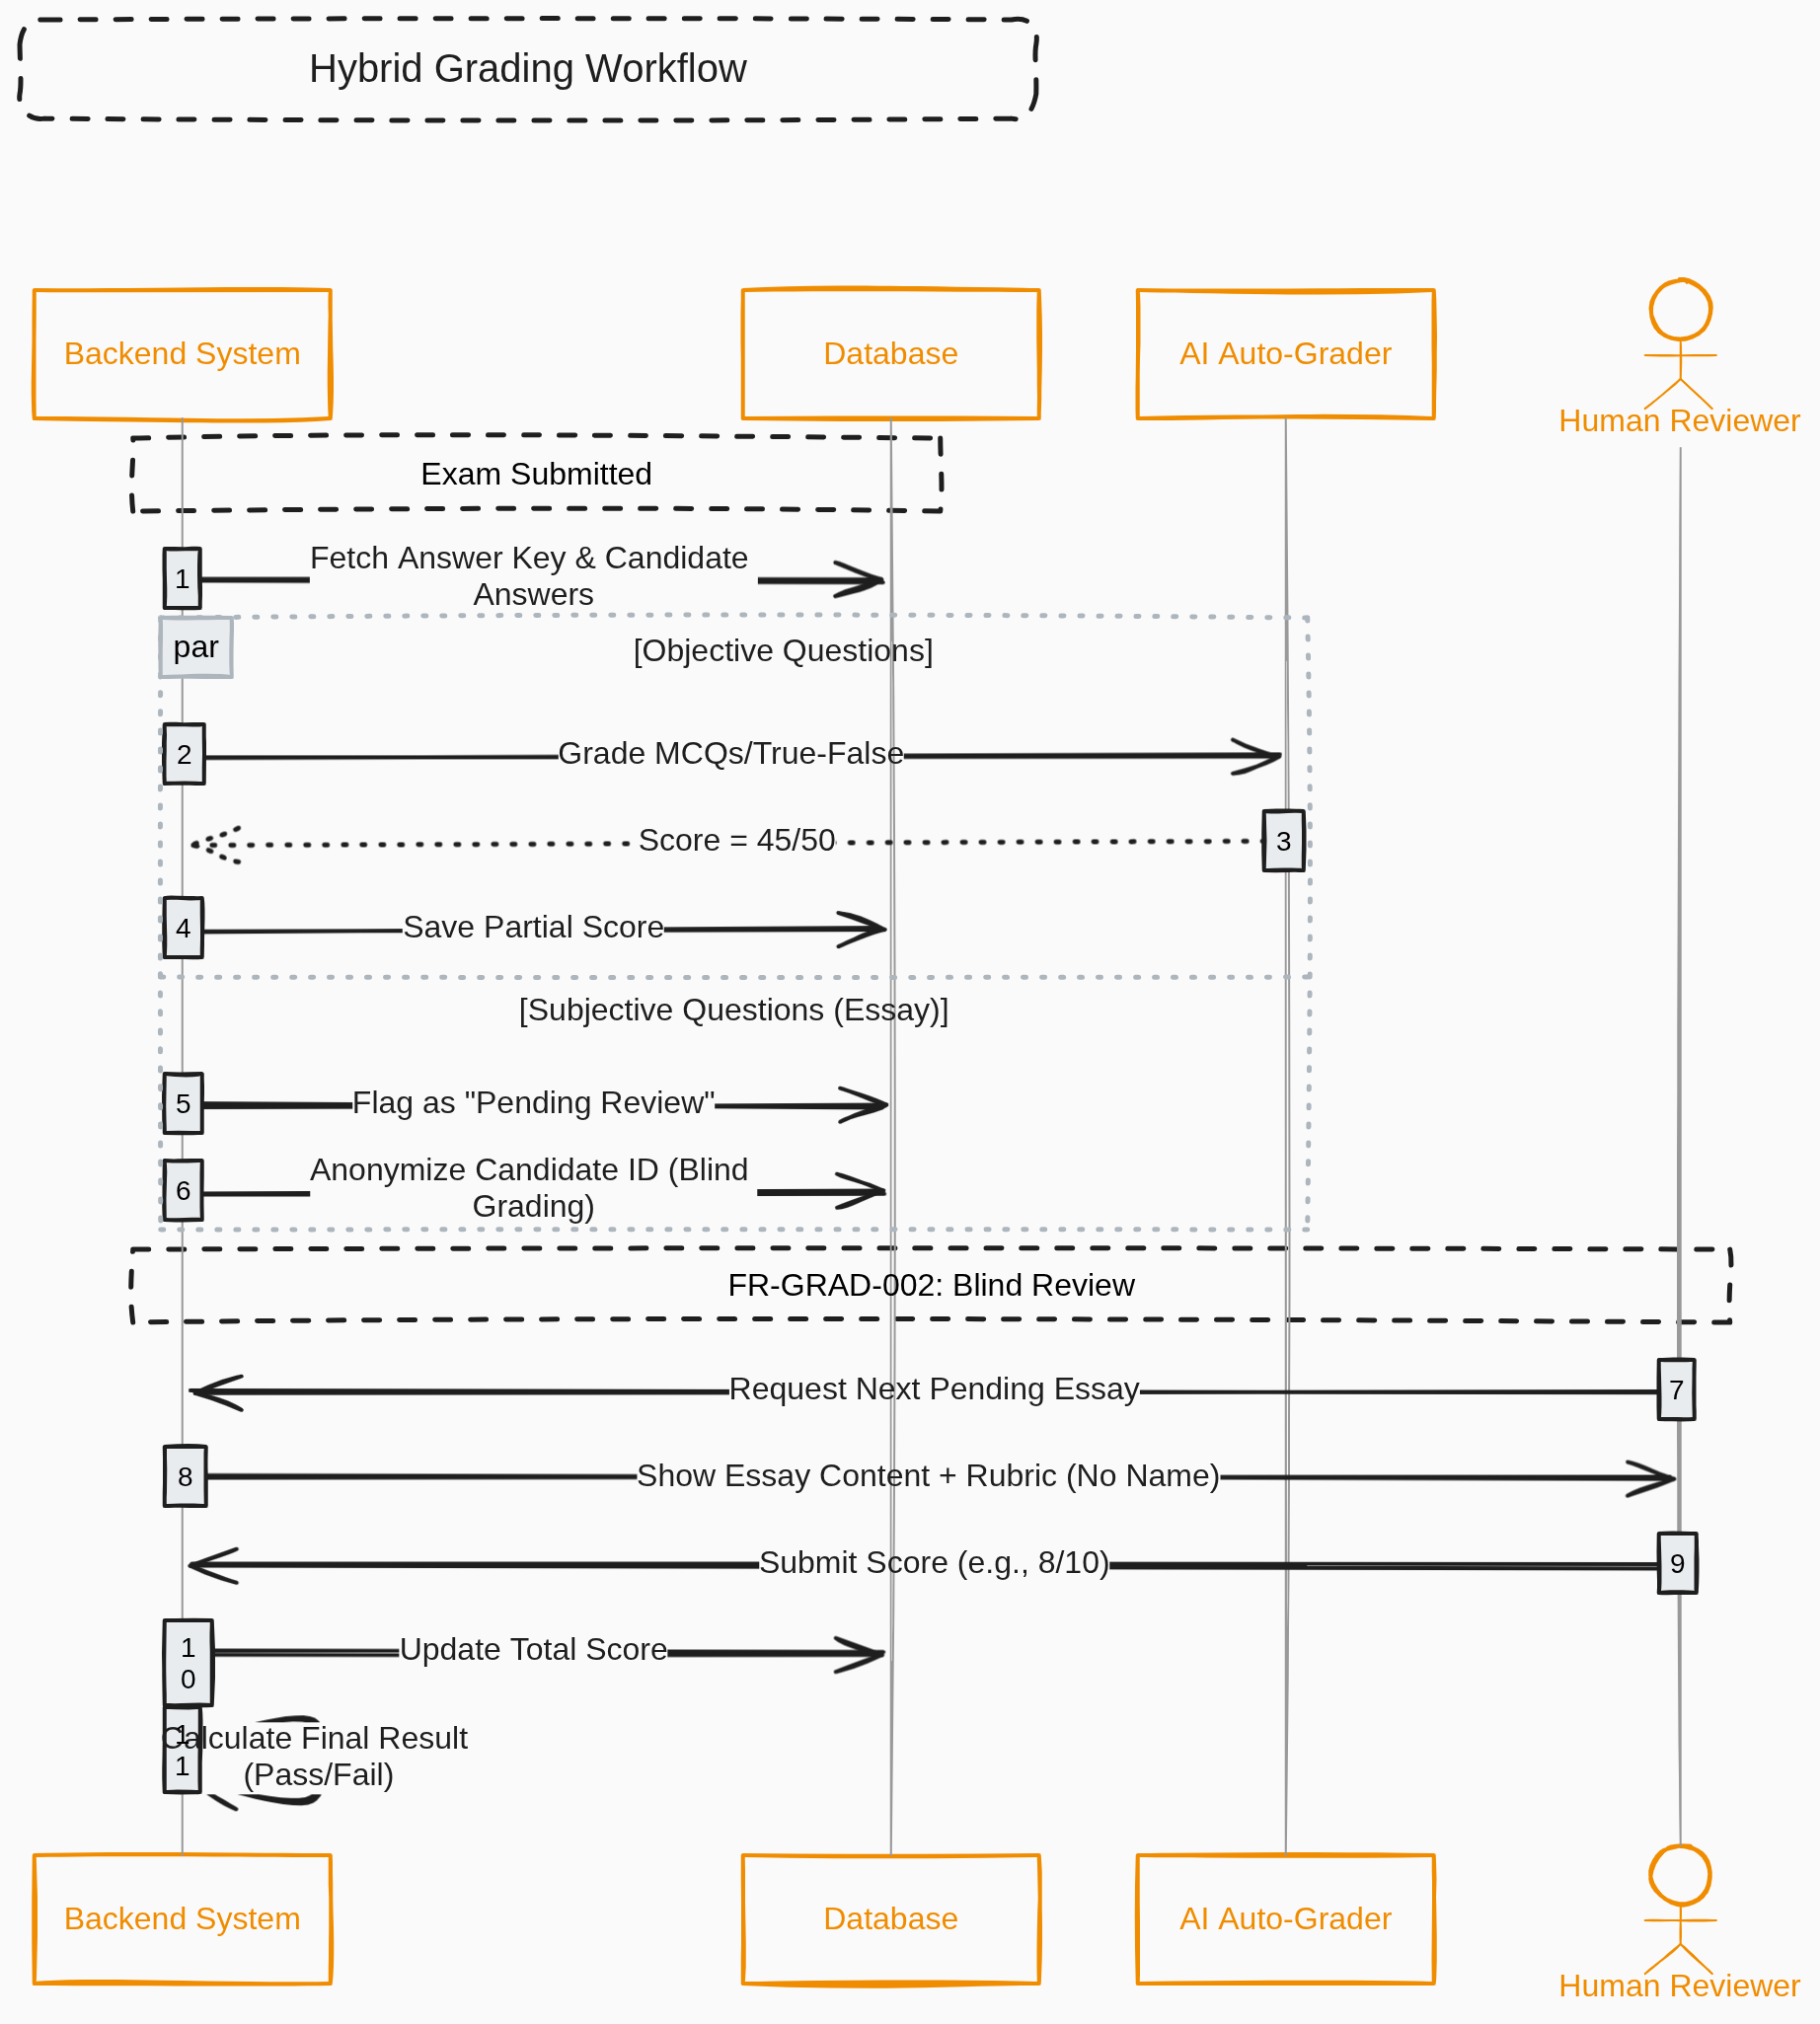
\includegraphics[width=0.9\textwidth]{assets/seq_diagrams/Hybrid Grading Workflow.png}
    \end{center}
    
    \textbf{Implements:} FR-GRAD-001, FR-GRAD-002 \\
    \textit{Split processing: Objective (auto-graded) + Subjective (blind human review)}
\end{frame}

\begin{frame}{SD: Async Report Generation}
    \begin{center}
        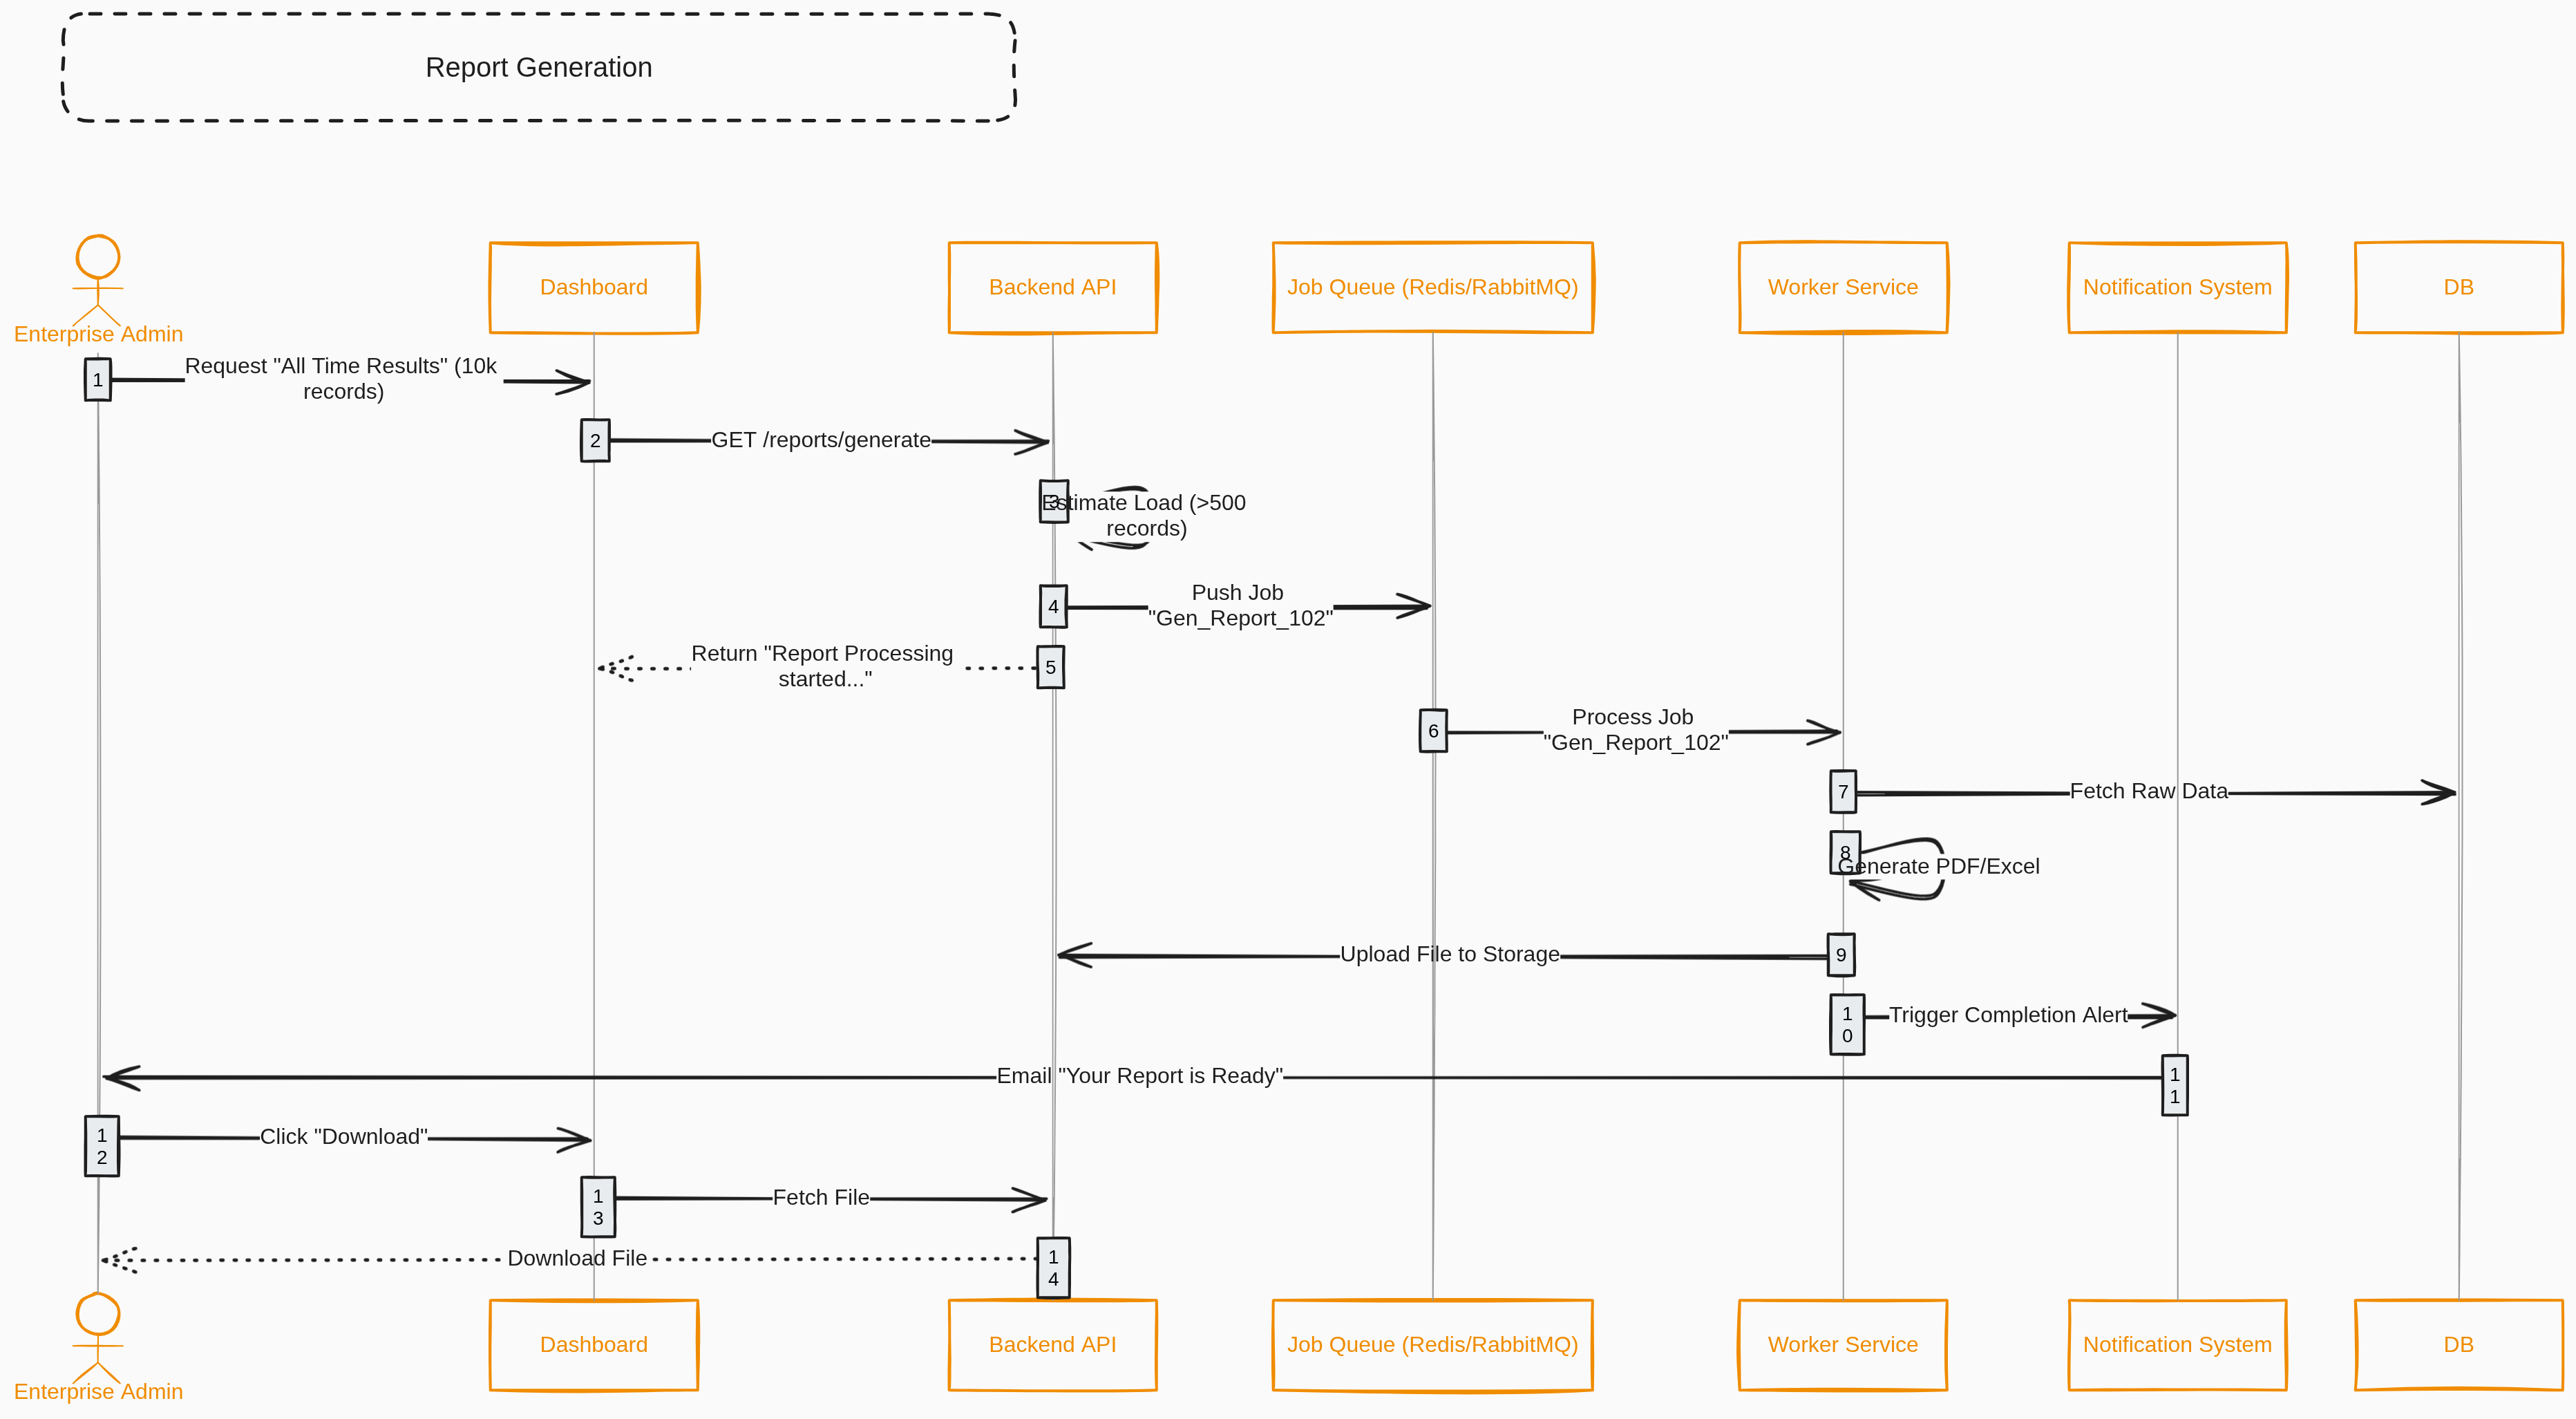
\includegraphics[width=0.9\textwidth]{assets/seq_diagrams/Report Generation.png}
    \end{center}
    
    \textbf{Implements:} FR-DASH-003 \\
    \textit{Performance optimization: Large reports ($\geq$500 records) offloaded to job queue, background processing}
\end{frame}

% =============================================================================
% Activity Diagrams
% =============================================================================
\begin{frame}{Activity Diagrams: Overview}
    \textbf{Activity diagrams model workflows, decision points, and parallel activities}
    
    \begin{block}{Four Main Workflows}
        \begin{enumerate}
            \item \textbf{Enterprise Registration \& Authentication}
            \begin{itemize}
                \item Organization registration → admin approval → subscription selection → payment → dashboard access
            \end{itemize}
            
            \item \textbf{Exam Creation \& Scheduling}
            \begin{itemize}
                \item Admin login → exam config (questions, duration, scoring, randomization) → candidate assignment → publish
            \end{itemize}
            
            \item \textbf{Candidate Exam + AI Proctoring}
            \begin{itemize}
                \item Candidate login → identity verification (facial) → exam with continuous AI monitoring → submission
            \end{itemize}
            
            \item \textbf{Grading + Certificate Generation}
            \begin{itemize}
                \item Submission received → auto-grade objective + manual blind-grade subjective → calculate score → analyze proctoring → certificate or flag
            \end{itemize}
        \end{enumerate}
    \end{block}
\end{frame}

\begin{frame}{AD: Enterprise Registration \& Authentication}
    \begin{center}
        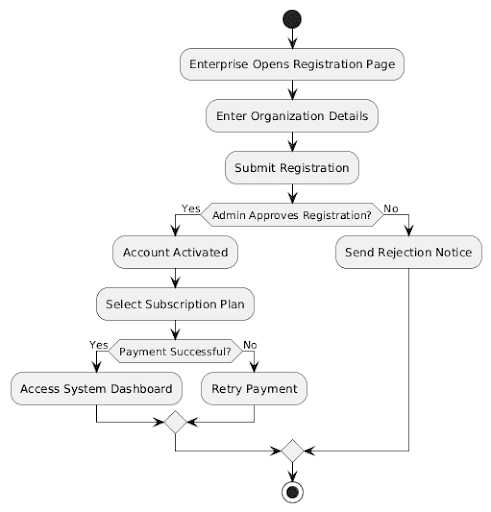
\includegraphics[width=0.9\textwidth]{assets/activity_diagrams/Enterprise Registration and Authentication.png}
    \end{center}
    
    \textit{Controlled system access with subscription enforcement}
\end{frame}

\begin{frame}{AD: Exam Creation \& Scheduling}
    \begin{center}
        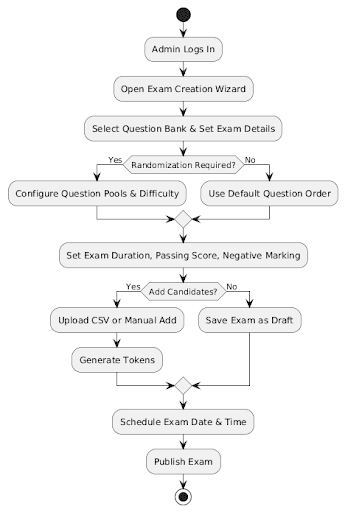
\includegraphics[width=0.7\textwidth]{assets/activity_diagrams/Exam Creation and Scheduling.png}
    \end{center}
    
    \textit{Flexible workflow supporting draft saving and immediate candidate assignment}
\end{frame}

\begin{frame}{AD: Candidate Exam + AI Proctoring}
    \begin{center}
        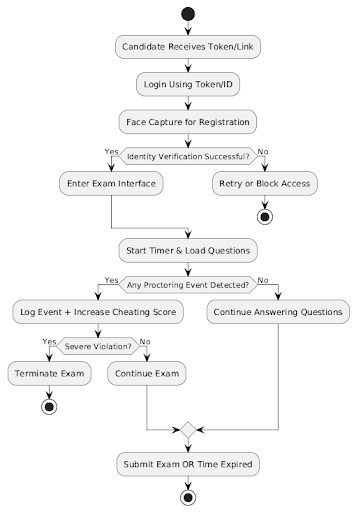
\includegraphics[width=0.65\textwidth]{assets/activity_diagrams/Candidate Exam and AI Proctoring.png}
    \end{center}
    
    \textit{Emphasizes exam integrity with real-time monitoring and violation handling}
\end{frame}

\begin{frame}{AD: Grading + Certificate Generation}
    \begin{center}
        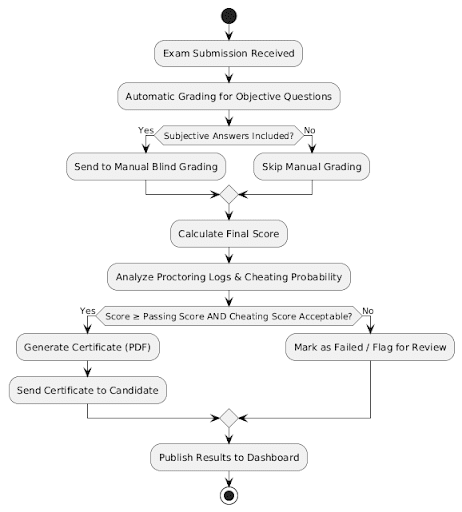
\includegraphics[width=0.7\textwidth]{assets/activity_diagrams/Grading and Certificate Generation.png}
    \end{center}
    
    \textit{Fair assessment ensuring both academic and integrity requirements}
\end{frame}

% =============================================================================
% Verification and Validation
% =============================================================================
\begin{frame}{System Model Verification \& Validation}
    \begin{block}{Requirements Validation}
        \begin{itemize}
            \item \textbf{Stakeholder Reviews:} Interactive sessions with HR managers, university administrators
            \item Confirmed requirements capture real-world needs (e.g., low-bandwidth resilience FR-CAND-005)
            \item \textbf{Prototyping:} Low-fidelity mockups validated usability requirements (FR-CAND-006)
        \end{itemize}
    \end{block}
    
    \begin{block}{Model Verification}
        \begin{itemize}
            \item \textbf{Consistency Checks:} Cross-verification between Use Case and Sequence diagrams
            \item Example: UC-08 Create Exam steps mapped to exam creation sequence diagram
            \item \textbf{Syntax Verification:} All UML diagrams verified against UML 2.5 standards
        \end{itemize}
    \end{block}
\end{frame}

\begin{frame}{Traceability Analysis}
    \begin{block}{Traceability Matrix (Sample)}
        \begin{table}[]
            \centering
            \small
            \begin{tabular}{|l|p{4cm}|p{4cm}|}
                \hline
                \textbf{Req. ID} & \textbf{Requirement Title} & \textbf{Implemented By (Use Case)} \\
                \hline
                FR-MT-002 & Enterprise Registration & UC-05: Register Enterprise \\
                \hline
                FR-MT-003 & Enterprise Account Approval & UC-01: Approve Enterprise Registration \\
                \hline
                FR-EXM-001 & Question Bank Management & UC-08: Create Exam \\
                \hline
                FR-EXM-003 & Strict Scheduling & UC-09: Schedule Exam \\
                \hline
                FR-CAND-006 & Accessibility & UC-18: Start Exam, UC-19: View Results \\
                \hline
                FR-GRAD-005 & Certificate Generation & UC-17: Receive Certificate \\
                \hline
            \end{tabular}
        \end{table}
    \end{block}
    
    \textit{Every critical requirement is addressed in system design}
\end{frame}
